\documentclass[10pt]{article}

\usepackage[table,xcdraw]{xcolor}
\usepackage[utf8]{inputenc}
\usepackage{tabularx}
\usepackage{hyperref}
\usepackage{array}
\usepackage{graphicx} % Per inserire immagini (loghi)
\usepackage{geometry} % Per personalizzare i margini
\usepackage{fancyhdr} % Per gestire intestazioni e piè di pagina
\usepackage{tikz}
\usepackage{ragged2e}
\usepackage{anyfontsize}
\usepackage{tabularx, etoolbox}
\usepackage{eso-pic} % Per aggiungere elementi grafici su tutte le pagine
\usepackage{float}
\usepackage{longtable}

\newcommand\version{2.0.0} %aggiunta versione come variabile

\graphicspath{{images/}}
%\graphicspath{{../images/}}

\setcounter{secnumdepth}{4}
\setcounter{tocdepth}{4}

%cambio misure della pagina
\geometry{a4paper,left=25mm,right=25mm,top=25mm,bottom=25mm}
\definecolor{colorePie}{HTML}{ebdfc7}
\pagestyle{fancy}
\fancyhf{}
\renewcommand{\headrulewidth}{0.4pt}
\lhead{
    \parbox[c]{1cm}{\includegraphics[width=1.1cm]{Sevenbitslogo.png}}
}
\rhead{\textcolor[HTML]{9e978a}{ PIANO DI QUALIFICA v\version}
}
\setlength{\headheight}{25pt}
\cfoot{\thepage}

\renewcommand*\contentsname{Indice}
\renewcommand{\listfigurename}{Elenco delle figure}
\renewcommand{\listtablename}{Elenco delle tabelle}

\begin{document}

% Pagina del titolo
\begin{titlepage}
    \setcounter{page}{0}
    \centering
    % Inserisci il logo del gruppo (modifica il percorso dell'immagine)
    \includegraphics[width=7.2cm]{Sevenbitslogo.png} \\[2cm]

    % Titolo
     {\fontsize{40}{40}\bfseries Piano di Qualifica}\selectfont \\[3.9em]

    % Sottotitolo
    {\huge NearYou\\ \vspace{3mm }Smart custom advertising platform} \\[2.7em]

    % Email del gruppo
    {\large sevenbits.swe.unipd@gmail.com} \\[3em]

    % Spazio per il logo dell'università
    \hfill

    \AddToShipoutPictureBG{ % Imposta il triangolo con logo
        \ifnum\value{page}=0
        \begin{tikzpicture}[overlay]

            % Definisce un triangolo blu in basso a destra
            \fill[colorePie]
                (current page.south east) -- ++(-9cm,0) -- ++(9cm,9cm);

            % Inserisce il logo all'interno del triangolo
            \node[anchor=south east, xshift=-0.3cm, yshift=0.3cm] at (current page.south east) {
                \includegraphics[width=4.5cm]{LogoUnipd.png}
            };
        \end{tikzpicture}
        \fi
    }

\vfill % Aggiunge spazio verticale per centrare il contenuto
\end{titlepage}
\newpage
\clearpage
\setcounter{page}{1}

% Registro Modifiche
\begin{center}
 \textbf{Registro modifiche}\\   
\end{center}

\renewcommand{\arraystretch}{1.5}
\rowcolors{0}{gray!11}{white} % Aggiunge colore alternato alle righe

\begin{longtable}{|>{\centering\arraybackslash}m{1.5cm}|>{\centering\arraybackslash}m{2cm}|>{\centering\arraybackslash}m{2.5cm}|>{\centering\arraybackslash}m{2.5cm}|>{\centering\arraybackslash}m{5cm}|}
\hline
\textbf{Versione} & \textbf{Data} & \textbf{Autore} & \textbf{Verificatore} & \textbf{Descrizione}\\
\endhead
    \hline
    2.0.0 & 2025-04-11 & Leonardo Trolese & Manuel Gusella & Approvazione documento per PB$_G$\\
    \hline
    1.2.1 & 2025-04-10 & Leonardo Trolese & Manuel Gusella & Aggiunta e analisi della restante parte dei grafici aggiornati\\
    \hline
    1.2.0 & 2025-04-09 & Federico Pivetta & Manuel Gusella & Aggiunta sezione per le metriche con sola misurazione finale\\
    \hline
    1.1.1 & 2025-04-08 & Leonardo Trolese & Manuel Gusella & Aggiunta e analisi di parte dei grafici aggiornati\\
    \hline
    1.1.0 & 2025-03-29 & Federico Pivetta & Riccardo Piva & Aggiunta sezione per le metriche escluse dal cruscotto$_G$\\
    \hline
    1.0.5 & 2025-03-28 & Leonardo Trolese & Riccardo Piva & Ampliamento del cruscotto$_G$ con le metriche relative alla revisione PB$_G$\\
    \hline
    1.0.4 & 2025-03-26 & Federico Pivetta & Riccardo Piva & Ampliamento del cruscotto$_G$ con le metriche relative alla revisione PB$_G$\\
    \hline
    1.0.3 & 2025-03-26 & Alfredo Rubino & Riccardo Piva & Redazione sottosezione Test$_G$ di Unità \\
    \hline
    1.0.2 & 2025-03-25 & Leonardo Trolese & Riccardo Piva & Aggiornamento metriche a seguito di inizio stesura codice \\
    \hline
    1.0.1 & 2025-03-21 & Federico Pivetta & Uncas Peruzzi & Correzione ai test$_G$ di sistema$_G$\\
    \hline
    1.0.0 & 2025-02-21 & Giovanni Cristellon & Leonardo Trolese & Approvazione documento per RTB$_G$\\
    \hline
    0.4.8 & 2025-02-21 & Leonardo Trolese & Manuel Gusella & Correzione errori minori\\
    \hline
    0.4.7 & 2025-02-18 & Leonardo Trolese & Pivetta Federico & Aggiunta ulteriori grafici sulle metriche del \hyperref[sec:cruscotto]{cruscotto di valutazione}\\
    \hline
    0.4.6 & 2025-02-16 & Leonardo Trolese & Pivetta Federico & Aggiunta ulteriori grafici sulle metriche del \hyperref[sec:cruscotto]{cruscotto di valutazione}\\
    \hline
    0.4.5 & 2025-02-15 & Leonardo Trolese & Pivetta Federico & Aggiunta grafici sulle metriche del \hyperref[sec:cruscotto]{cruscotto di valutazione}\\ 
    \hline
    0.4.4 & 2025-02-11 & Federico Pivetta & Uncas Peruzzi & Correzione ai test$_G$ di sistema$_G$ e di accettazione a seguito delle modifiche all'Analisi dei Requisiti\\
    \hline
    0.4.3 & 2025-01-14 & Federico Pivetta & Leonardo Trolese & Riorganizzazione delle metriche di qualità\\
    %\hline
    %0.4.3 & 2025-01-10 & Leonardo Trolese & Uncas Peruzzi & Aggiunta dei test$_G$ di integrazione\\
    \hline
    0.4.2 & 2025-01-10 & Federico Pivetta & Leonardo Trolese & Aggiunta dei test$_G$ di sistema$_G$ e dei test$_G$ di accettazione\\
    \hline
    0.4.1 & 2025-01-08 & Riccardo Piva & Uncas Peruzzi & Refactor generale sezione qualità processo$_G$ e qualità prodotto \\
    \hline
    0.4.0 & 2025-01-07 & Riccardo Piva & Uncas Peruzzi & Creazione cruscotto$_G$\\
    \hline
    0.3.3 & 2025-01-03 & Riccardo Piva & Uncas Peruzzi & Correzioni minori generali \\
    \hline
    0.3.2 & 2024-12-16 & Alfredo Rubino & Manuel Gusella & Aggiunta acronimi metriche e correzioni minori\\
    \hline
    0.3.1 & 2024-12-13 & Riccardo Piva & Alfredo Rubino & Correzione standard IEEE$_G$ \\
    \hline
    0.3.0 & 2024-12-12 & Riccardo Piva & Alfredo Rubino & Arricchimento sezioni Qualità di processo$_G$, Qualità di prodotto e inizio redazione modalità testing \\
    \hline
    0.2.0 & 2024-12-06 & Manuel Gusella  & Alfredo Rubino & Inizio redazione sottosezione Qualità di prodotto\\
    \hline
    0.1.0 & 2024-11-21 & Uncas Peruzzi  & Federico Pivetta & Inizio redazione del documento\\
    \hline
\end{longtable}
\rowcolors{0}{}{} % Riporta le righe alla colorazione originale

\newpage
\tableofcontents
\newpage
\listoffigures %elenco delle figure sarà da usare per ogni immagine
\newpage
\listoftables %lista delle tabelle presenti nel documento
\newpage
\begin{justify}

\section{Introduzione}

\subsection{Scopo del documento}
Il seguente documento ha l'obiettivo di garantire la qualità del prodotto e dei processi coinvolti nell'intero progetto$_G$. Al fine di assicurare che il prodotto soddisfi le aspettative di qualità attese, il documento
verrà aggiornato nel tempo per riflettere eventuali modifiche, integrazioni e i risultati delle verifiche effettuate.


\subsection{Glossario}
Con l'intento di evitare ambiguità nell'interpretazione del linguaggio utilizzato, viene fornito un glossario che si occupa di esplicitare il significato dei termini che riguardano il contesto del progetto$_G$. I termini presenti nel glossario sono contrassegnati con una $_G$ a pedice : Termine$_G$.\\
Le definizioni sono contenute nell'apposito documento \textit{Glossario}.\\


\subsection{Riferimenti}


\subsubsection{Riferimenti normativi}
\begin{itemize}
    \item[-] \textit{Norme\_di\_Progetto\_v1.0.0}

    \item[-] Regolamento del progetto$_G$ didattico  \\
      \textcolor{blue}{\texttt{\url{https://www.math.unipd.it/~tullio/IS-1/2024/Dispense/PD1.pdf}}}\\
      (Consultato: 2025-02-19).
    \item[-] Capitolato$_G$ C4 - NearYou - Smart custom advertising platform\\
    \textcolor{blue}{\texttt{\url{https://www.math.unipd.it/~tullio/IS-1/2024/Progetto/C4p.pdf}}}\\
    (Consultato: 2025-02-19).\\
    \textcolor{blue}{\texttt{\url{https://www.math.unipd.it/~tullio/IS-1/2024/Progetto/C4.pdf}}}\\
    (Consultato: 2025-02-19).
    
    \item[-] Standard ISO/IEC 9126 \label{ISO 9126} \\
    \textcolor{blue}{\texttt{\url{https://en.wikipedia.org/wiki/ISO/IEC_9126}}}\\
    (Consultato: 2025-02-19).
    \item[-] Standard ISO/IEC/IEEE 12207:1995 \label{ISO 12207:1995}\\
    \textcolor{blue}{\texttt{\url{https://www.math.unipd.it/~tullio/IS-1/2009/Approfondimenti/ISO_12207-1995.pdf}}}\\
    (Consultato: 2025-02-19).

\end{itemize}
\subsubsection{Riferimenti informativi}
\begin{itemize}
    \item[-] Qualità di prodotto\\
    \textcolor{blue}{\texttt{\url{https://www.math.unipd.it/~tullio/IS-1/2024/Dispense/T07.pdf}}}\\
    (Consultato: 2025-02-19).
    \item[-] Qualità di processo$_G$\\
    \textcolor{blue}{\texttt{\url{https://www.math.unipd.it/~tullio/IS-1/2024/Dispense/T08.pdf}}}\\
    (Consultato: 2025-02-19).
    \item[-] Verifica e validazione\\
    \textcolor{blue}{\texttt{\url{https://www.math.unipd.it/~tullio/IS-1/2024/Dispense/T09.pdf}}}\\
    (Consultato: 2025-02-19).\\
    \textcolor{blue}{\texttt{\url{https://www.math.unipd.it/~tullio/IS-1/2024/Dispense/T10.pdf}}}\\
    (Consultato: 2025-02-19).\\
    \textcolor{blue}{\texttt{\url{https://www.math.unipd.it/~tullio/IS-1/2024/Dispense/T11.pdf}}}\\
    (Consultato: 2025-02-19).
\end{itemize}
\newpage

\section{Obiettivi metrici di qualità}
Per far sì che un prodotto raggiunga uno standard qualitativo, è necessario definire delle metriche precise che permettano di monitorare e indicare il grado di qualità del prodotto e che quindi permettano di definire questo standard.
Queste metriche vengono definite nel documento \textit{Norme di Progetto}.
Questa sezione si occuperà di definire i parametri di accettazione e ottimalità delle relative metriche.\\

\subsection{Qualità di prodotto}
La qualità di prodotto è intesa come valutazione del software, e più precisamente per la determinazione del grado di conformità alle attese.\\
Si rivolge l'attenzione su aspetti come Usabilità, Affidabilità e Manutenibilità, ma più in generale alla qualità esterna (funzionale) ed interna (strutturale) del prodotto software.\\
Quindi non basta che il software implementi le funzionalità richieste dal proponente$_G$, ma le esegua secondo specifici standard di qualità.\\
In seguito sono presenti le metriche definite dallo \hyperref[ISO 9126]{standard ISO/IEC 9126} che il gruppo si impegna a soddisfare per la qualità del prodotto software.
\subsubsection{Funzionalità}
\begin{table}[H]
  \centering
\begin{tabular}{|c|c|c|c|}
  \hline
  \textbf{Metrica} & \textbf{Descrizione} & \textbf{Valore accettazione} & \textbf{Valore ideale}\\
  \hline
  MPD01 & Requisiti Obbligatori Soddisfatti & 100\% & 100\%\\
  \hline
  MPD02 & Requisiti Desiderabili Soddisfatti  & $\geq$ 0\% & 100\% \\
  \hline
  MPD03 & Requisiti Opzionali Soddisfatti & $\geq$ 0\% & 100\% \\
  \hline
\end{tabular}
\caption{Funzionalità - Qualità di prodotto}
\label{tab:funzionalità}
\end{table}

\subsubsection{Affidabilità}
\begin{table}[H]
  \centering
\begin{tabular}{|c|c|c|c|}
  \hline
  \textbf{Metrica} & \textbf{Descrizione} & \textbf{Valore accettazione} & \textbf{Valore ideale}\\
  \hline
  MPD04 & Line coverage & $\geq$ 80\% & 100\% \\
  \hline
  % MPD06 & Statement coverage & $\geq$ 80\% & 100\% \\
  % \hline
  MPD05 & Branch$_G$ coverage & $\geq$ 80\% & 100\% \\
  \hline
  % MPD08 & Condition coverage & $\geq$ 80\% & 100\% \\
  % \hline
\end{tabular}
\caption{Affidabilità - Qualità di prodotto}
\label{tab:affidabilità}
\end{table}

\subsubsection{Efficienza}
\begin{table}[H]
  \centering
\begin{tabular}{|c|c|c|c|}
  \hline
  \textbf{Metrica} & \textbf{Descrizione} & \textbf{Valore accettazione} & \textbf{Valore ideale}\\
  \hline
  MPD06 & Tempo medio di risposta & $\leq$ 10 secondi & $\leq$ 4 secondi \\
  \hline
\end{tabular}
\caption{Efficienza - Qualità di prodotto}
\label{tab:efficienza}
\end{table}

\subsubsection{Usabilità}
\begin{table}[H]
  \centering
\begin{tabular}{|c|c|c|c|}
  \hline
  \textbf{Metrica} & \textbf{Descrizione} & \textbf{Valore accettazione} & \textbf{Valore ideale}\\
  \hline
  MPD07 & Facilità di utilizzo & $\leq$ 7 click & $\leq$ 5 click\\
  \hline
  MPD08 & Tempo medio di apprendimento & $\leq$ 5 minuti & $\leq$ 2 minuti \\
  \hline
\end{tabular}
\caption{Usabilità - Qualità di prodotto}
\label{tab:usabilità}
\end{table}

\subsubsection{Manutenibilità}
\begin{table}[H]
  \centering
\begin{tabular}{|c|c|c|c|}
  \hline
  \textbf{Metrica} & \textbf{Descrizione} & \textbf{Valore accettazione} & \textbf{Valore ideale}\\
  % \hline
  % MPD12 & Coefficiente di accoppiamento fra classi & $\leq$ 4 & $\leq$ 2 \\
  \hline
  MPD09 & Linee di codice per metodo & $\leq$ 50 & $\leq$ 25 \\
  % \hline
  % MPD10 & Parametri per metodo & $\leq$ 7 & $\leq$ 4 \\
  \hline
  MPD10 & Attributi per classe & $\leq$ 7 & $\leq$ 5 \\
  \hline
  MPD11 & Structure Fan IN & - & - \\
  \hline
  MPD12 & Structure Fan OUT & - & va minimizzato \\
  \hline
\end{tabular}
\caption{Manutenibilità - Qualità di prodotto}
\label{tab:manutenibilità}
\end{table}

\subsubsection{Portabilità}
\begin{table}[H]
  \centering
\begin{tabular}{|c|c|c|c|}
  \hline
  \textbf{Metrica} & \textbf{Descrizione} & \textbf{Valore accettazione} & \textbf{Valore ideale}\\
  \hline
  MPD13 & Versioni browser supportati & $\geq$ 80\% & 100\% \\
  \hline
\end{tabular}
\caption{Portabilità - Qualità di prodotto}
\label{tab:portabilità}
\end{table}


\subsection{Qualità di processo}
La qualità di processo$_G$ è intesa come valutazione delle attività svolte per la realizzazione del prodotto.\\
Seguendo delle buone pratiche e delle linee guida nello sviluppo software, si può garantire che il prodotto finale avrà rispettato a sua volta degli standard qualitativi rendendolo così un prodotto di qualità.\\
Qui sotto divideremo le metriche di qualità di processo$_G$ seguendo lo \hyperref[ISO 12207:1995]{standard ISO/IEC 12207:1995} in tre categorie: Processi primari, Processi di supporto e Processi organizzativi.\\
\subsubsection{Processi Primari}
I processi primari si possono dividere in parti primarie e una parte primaria è quella che inizia o esegue lo sviluppo, l'operazione o la manutenzione di prodotti software.\\

\paragraph{Fornitura}\mbox{}\\
La fornitura è il processo$_G$ che si occupa di consegnare il prodotto software al cliente.\\
Serve per garantire che il prodotto soddisfi i requisiti di tempi e costi definiti con il cliente.\\
\begin{table}[H]
\centering
\begin{tabular}{|>{\centering\arraybackslash}p{1.5cm}|>{\centering\arraybackslash}p{5cm}|>{\centering\arraybackslash}p{4cm}|>{\centering\arraybackslash}p{3.7cm}|}
  \hline
  \textbf{Metrica} & \textbf{Descrizione} & \textbf{Valore accettazione} & \textbf{Valore ideale}\\
  \hline
  MPC01 & Estimated at completion (EAC) & \textpm5\% rispetto al (BAC)\(_G\) & Budget at completion (BAC)\(_G\)\\
  \hline
  MPC02 & Estimate to complete (ETC) & $\geq$ 0 & $\leq$ EAC$_G$\(_G\) \\
  \hline
  MPC03 & Actual cost (AC) & $\geq$ 0 & $\leq$ EAC$_G$\(_G\) \\
  \hline
  MPC04 & Earned value (EV) & $\geq$ 0 & $\leq$ EAC$_G$\(_G\) \\
  \hline
  MPC05 & Planned value (PV) & $\geq$ 0 & $\leq$ Budget at completion (BAC)\(_G\) \\
  \hline
  MPC06 & Schedule variance (SV) & $\geq$ -5\% rispetto al (BAC)\(_G\) & $\geq$ 0\% \\
  \hline
  MPC07 & Cost variance (CV) & $\geq$ -5\% rispetto al (BAC)\(_G\) & $\geq$ 0\% \\
  \hline
  MPC08 & Cost Performance Index (CPI) & $\geq$ 0.9 & $\geq$ 1.0 \\
  \hline
\end{tabular}
\caption{Processi primari - Fornitura}
\label{tab:fornitura}
\end{table}

\paragraph{Sviluppo}\mbox{}\\
Lo sviluppo è il processo$_G$ riguardante la scrittura del codice del prodotto software.\\
Questa metrica serve a garantire che il software rispetti le richieste del cliente e che la codifica avvenga in modo efficiente\\
\begin{table}[H]
  \centering
\begin{tabular}{|c|c|c|c|}
  \hline
  \textbf{Metrica} & \textbf{Descrizione} & \textbf{Valore accettazione} & \textbf{Valore ideale}\\
  \hline
  MPC09 & Requisiti Obbligatori Soddisfatti (ROS) & 100\% & 100\%\\
  \hline
  MPC10 & Requirements Stability Index (RSI) & $\geq$ 80\% & 100\% \\
  \hline
\end{tabular}
\caption{Processi primari - Codifica}
\label{tab:codifica}
\end{table}


\subsubsection{Processi di Supporto}
Un processo$_G$ di supporto è un processo$_G$ che supporta un altro processo$_G$ come parte integrante con uno scopo distinto e contribuisce al successo e alla qualità del progetto$_G$ software.\\
Un processo$_G$ di supporto è impiegato ed eseguito, se necessario, da un altro processo$_G$.\\
\paragraph{Documentazione}\mbox{}\\
La documentazione$_G$ è essenziale per la comprensione del prodotto e per la sua manutenzione.\\
Di conseguenza è essenziale che questa sia chiara, comprensibile e corretta.\\
\begin{table}[H]
  \centering
\begin{tabular}{|c|c|c|c|}
  \hline
  \textbf{Metrica} & \textbf{Descrizione} & \textbf{Valore accettazione} & \textbf{Valore ideale}\\
  \hline
  MPC11 & Indice Gulpease & $\geq$ 40\% & $\geq$ 60\% \\
  \hline
  MPC12 & Correttezza ortografica & 0 errori & 0 errori \\
  \hline
\end{tabular}
\caption{Processi di supporto - Documentazione}
\label{tab:documentazione}
\end{table}

\paragraph{Verifica}\mbox{}\\
La verifica serve a garantire che il prodotto software sia conforme alle specifiche e non contenga errori.\\
\begin{table}[H]
  \centering
\begin{tabular}{|c|c|c|c|}
  \hline
  \textbf{Metrica} & \textbf{Descrizione} & \textbf{Valore accettazione} & \textbf{Valore ideale}\\
  \hline
  MPC13 & Line coverage & $\geq$ 80\% & 100\% \\
  \hline
  MPC14 & Passed test$_G$ cases percentage & $\geq$ 80\% & 100\% \\
  \hline
\end{tabular}
\caption{Processi di supporto - Verifica}
\label{tab:verifica}
\end{table}

\paragraph{Gestione della qualità}\mbox{}\\
La gestione della qualità è necessaria per garantire che tutte le metriche di qualità vengano effettivamente soddisfatte.\\
\begin{table}[H]
  \centering
\begin{tabular}{|c|c|c|c|}
  \hline
  \textbf{Metrica} & \textbf{Descrizione} & \textbf{Valore accettazione} & \textbf{Valore ideale}\\
  \hline
  MPC15 & Metriche di qualità soddisfate & $\geq$ 85\% & 100\% \\
  \hline
\end{tabular}
\caption{Processi di supporto - Gestione della qualità}
\label{tab:gestione della qualità}
\end{table}

\subsubsection{Processi Organizzativi}
I processi organizzativi servono per creare un sottostruttura per il ciclo-di-vita$_G$ e
per garantire che i processi principali e i loro processi di supporto siano ben strutturati e vengano continuamente migliorati.\\
\paragraph{Gestione dei processi}\mbox{}\\
La gestione dei processi indica come vengono gestiti i processi all'interno del progetto$_G$.\\
\begin{table}[H]
  \centering
\begin{tabular}{|c|c|c|c|}
  \hline
  \textbf{Metrica} & \textbf{Descrizione} & \textbf{Valore accettazione} & \textbf{Valore ideale}\\
  \hline
  MPC16 & Rischi non previsti & $\leq$ 3 & 0 \\
  \hline
  MPC17 & Efficienza$_G$ temporale (ET) & $\leq$ 5.0 & $\geq$ 1.0 \\
  \hline
\end{tabular}
\caption{Processi organizzativi - Gestione dei processi}
\label{tab:gestione dei processi}
\end{table}
\newpage

\section{Modalità di Testing}
Qui sotto sono elencati i vari test$_G$ che vengono eseguiti automaticamente sul prodotto software.\\
Questo serve a garantire che il prodotto soddisfi i requisiti e le aspettative indicate nel documento \textit{Analisi dei Requisiti}.\\
I test$_G$ sono divisi in quattro categorie: Test$_G$ di unità, Test$_G$ di sistema$_G$, Test$_G$ di integrazione e Test$_G$ di accettazione.\\
Per indicarne lo stato, come definito nel documento \textit{Norme di Progetto} vengono utilizzate le seguenti abbreviazioni:
\begin{itemize}
\item \textbf{P}: Passato
\item \textbf{NP}: Non Passato
\item \textbf{NI}: Non Implementato
\end{itemize}

\subsection{Test di unità}
I test$_G$ di unità servono a verificare che ogni singola unità del software funzioni correttamente.\\

\begin{longtable}{|>{\centering\arraybackslash}m{2cm}|>{\centering\arraybackslash}m{7cm}|>{\centering\arraybackslash}m{2cm}|>{\centering\arraybackslash}m{2cm}|}
\hline
\textbf{Codice} & \textbf{Descrizione} & \textbf{Stato}\\
\endhead
\hline
TU1 & Verificare che la classe \texttt{ClickhouseActivityRepository} restituisca correttamente le attività entro un determinato raggio geografico e i dettagli di una specifica attività a partire dal nome. Se l'attività non viene trovata, deve restituire un oggetto vuoto. & P \\
\hline
TU2 & Verificare che la classe \texttt{ClickhouseMessageRepository} restituisca correttamente l'ultimo messaggio inviato da un utente, includendo tutte le informazioni associate. In caso di assenza di messaggi, deve restituire un oggetto vuoto con valori di default. & P \\
\hline
TU3 & Verificare che la classe \texttt{ClickhouseUserRepository} gestisca correttamente l'assegnazione e il recupero delle informazioni sugli utenti. In particolare, deve aggiornare lo stato di un utente come occupato, recuperare un utente libero, restituire i dettagli di un utente associato a un sensore e gestire correttamente i casi in cui nessun utente venga trovato. & P \\
\hline
TU4 & Verificare che la classe \texttt{CustomPrompt} generi correttamente un prompt formattato in base alle informazioni dell'utente e alle attività disponibili. Deve garantire che i dati forniti siano integrati correttamente nel testo generato e che venga mantenuta una struttura valida anche in caso di dati mancanti. & P \\
\hline
TU5 & Verificare che la classe \texttt{DatabaseConnection} gestisca correttamente la connessione e la disconnessione al database$_G$. Inoltre, si verifica che la classe \texttt{DatabaseConfigParameters} inizializzi correttamente i valori di default dei parametri di configurazione. & P \\
\hline
TU6 & Verificare che le classi DTO (\texttt{MessageDTO}, \texttt{UserDTO}, \texttt{ActivityDTO}) inizializzino correttamente i dati forniti e gestiscano i valori di default quando i parametri non vengono specificati. & P \\
\hline
TU7 & Verificare che la classe \texttt{FilterMessageAlreadyDisplayed} filtri correttamente i messaggi già visualizzati dall'utente, escludendo i messaggi con le stesse coordinate dell'ultimo messaggio inviato, i messaggi con coordinate (0,0) e quelli che risultano identici dopo l'arrotondamento delle coordinate. & P \\
\hline
TU8 & Verificare che la classe \texttt{FlinkJobManager} inizializzi e gestisca correttamente il flusso di dati in Apache Flink$_G$. Deve configurare correttamente le operazioni di \texttt{map} e \texttt{filter}, collegarsi a sorgenti e sink e avviare l'esecuzione del job tramite \texttt{execute}. & P \\
\hline
TU9 & Verificare che la classe \texttt{GroqLLMService} gestisca correttamente l'inizializzazione, la configurazione della chat e la generazione di risposte strutturate. In particolare, deve caricare la chiave API$_G$ dall'ambiente, impostare correttamente il modello \texttt{ChatGroq} con i parametri previsti e restituire un output coerente con la richiesta ricevuta. & P \\
\hline
TU10 & Verificare che la classe \texttt{JsonRowDeserializationAdapter} inizializzi correttamente lo schema di deserializzazione JSON$_G$, memorizzando correttamente il tipo di dati fornito e creando un'istanza di \texttt{JsonRowDeserializationSchema} con i parametri appropriati. & P \\
\hline
TU11 & Verificare che la classe \texttt{JsonRowSerializationAdapter} inizializzi correttamente lo schema di serializzazione JSON$_G$. In particolare, deve memorizzare il tipo di dati fornito e creare un'istanza di \texttt{JsonRowSerializationSchema} configurata con i parametri appropriati. & P \\
\hline
TU12 & Verificare che la classe \texttt{KafkaMessageWriter} inizializzi correttamente il writer Kafka$_G$. In particolare, deve configurare lo schema di serializzazione, impostare i parametri del sink Kafka$_G$ e restituire correttamente l'istanza del writer tramite il metodo \texttt{get\_message\_writer}. & P \\
\hline
TU13 & Verificare che la classe \texttt{KafkaPositionReceiver} configuri correttamente la sorgente Kafka$_G$. In particolare, deve impostare i parametri di connessione, il gruppo di consumo, il deserializzatore e le proprietà di gestione degli offset, restituendo correttamente l'istanza della sorgente tramite il metodo \texttt{get\_position\_receiver}. & P \\
\hline
TU14 & Verificare che la classe \texttt{KafkaSourceConfiguration} inizializzi correttamente i parametri di configurazione con i valori di default previsti, inclusi server, topic$_G$, gruppo di consumo e gestione degli offset. & P \\
\hline
TU15 & Verificare che la classe \texttt{KafkaWriterConfiguration} inizializzi correttamente i parametri di configurazione con i valori di default previsti. In particolare, deve garantire che il server, il topic$_G$ scrivibile e la struttura del \texttt{key\_type} siano definiti correttamente. & P \\
\hline
TU16 & Verificare che la classe \texttt{MessageSerializer} crei correttamente un oggetto \texttt{Row} a partire da un'istanza di \texttt{MessageDTO}. In particolare, deve garantire che i dati siano convertiti correttamente e mantenere la struttura prevista con il numero corretto di campi. & P \\
\hline
TU17 & Verificare che la classe \texttt{PositionToMessageProcessor} elabori correttamente le posizioni degli utenti e generi messaggi pubblicitari basati sulle attività nelle vicinanze. In particolare, deve gestire i casi in cui non ci siano attività disponibili e interagire con i repository$_G$ e il servizio AI per elaborare i dati. & P \\
\hline
TU18 & Verificare che la classe \texttt{BycicleSimulationStrategy} inizializzi correttamente i parametri di simulazione e calcoli correttamente il percorso$_G$, la velocità e il tempo tra le posizioni. In particolare, deve interagire con il grafo per ottenere un percorso$_G$ valido e restituire valori coerenti per velocità e intervallo di tempo. & P \\
\hline
TU19 & Verificare che la classe \texttt{DatabaseConfigParameters} inizializzi correttamente i parametri di configurazione con i valori di default previsti. & P \\
\hline
TU20 & Verificare che la classe \texttt{DatabaseConnection} gestisca correttamente la connessione e la disconnessione dal database$_G$. & P \\
\hline
TU21 & Verificare che la classe \texttt{GeoPosition} inizializzi correttamente i parametri e restituisca i valori attesi tramite i metodi di accesso. In particolare, deve garantire che \texttt{sensor\_id}, latitudine, longitudine e timestamp siano correttamente memorizzati e recuperabili. & P \\
\hline
TU22 & Verificare che la classe \texttt{GpsSensor} gestisca correttamente la simulazione della posizione. In particolare, deve inizializzare correttamente i parametri, generare e inviare posizioni simulate basate sulla strategia di simulazione e restituire i valori attesi per identificativo del sensore e tempo di aggiornamento. & P \\
\hline
TU23 & Verificare che la classe \texttt{GraphWrapper} inizializzi e recuperi correttamente la mappa stradale utilizzando \texttt{osmnx}. In particolare, deve chiamare \texttt{graph\_from\_point} con i parametri corretti per ottenere il grafo stradale basato sulla posizione, il raggio e il tipo di rete specificati. & P \\
\hline
TU24 & Verificare che la classe \texttt{KafkaConfigParameters} inizializzi correttamente i parametri di configurazione con i valori di default previsti, inclusi il server Kafka$_G$ e il topic$_G$ di origine. & P \\
\hline
TU25 & Verificare che la classe \texttt{KafkaConfluentAdapter} invii correttamente i dati al broker$_G$ Kafka$_G$. In particolare, deve serializzare correttamente le posizioni, produrre i messaggi con la chiave corretta e gestire la sincronizzazione dei thread tramite un meccanismo di lock. & P \\
\hline
TU26 & Verificare che la classe \texttt{PositionJsonAdapter} serializzi correttamente un oggetto \texttt{GeoPosition} in formato JSON$_G$, mantenendo la struttura e i valori attesi per identificativo, coordinate e timestamp. & P \\
\hline
TU27 & Verificare che la classe \texttt{SensorFactory} crei correttamente istanze di \texttt{GpsSensor}. In particolare, deve garantire che ogni sensore sia un'istanza valida di \texttt{SensorSubject} e \texttt{GpsSensor}, che gli UUID assegnati siano validi e univoci, e che il metodo per la creazione di una lista di sensori generi il numero corretto di istanze. & P \\
\hline
TU28 & Verificare che la classe \texttt{SensorRepository} gestisca correttamente l'assegnazione e il recupero dei sensori. In particolare, deve aggiornare lo stato di un sensore come occupato e recuperare un sensore non occupato dal database$_G$. & P \\
\hline
TU29 & Verificare che la classe \texttt{SensorSimulationAdministrator} gestisca correttamente l'avvio della simulazione dei sensori. In particolare, deve inizializzare correttamente il registro dei sensori, avviare la simulazione tramite un \texttt{ThreadPool} e gestire eventuali errori durante l'esecuzione. & P \\
\hline
TU30 & Verificare che la classe \texttt{UserRepository} gestisca correttamente l'assegnazione e il recupero degli utenti. In particolare, deve aggiornare lo stato di un utente come occupato e recuperare un utente libero dal database$_G$. & P \\
\hline
TU31 & Verificare che la classe \texttt{UserSensorService} assegni correttamente un sensore a un utente disponibile. In particolare, deve recuperare un utente e un sensore non occupati, aggiornare il loro stato nel database$_G$ e gestire correttamente i casi in cui non siano disponibili utenti o sensori. & P \\
\hline
\caption{Test di unità}\\
\end{longtable}


\subsection{Test di sistema}
I test$_G$ di sistema$_G$ servono a verificare la completa copertura dei requisiti concordati nel documento \textit{Analisi dei Requisiti}.\\

\begin{longtable}{|>{\centering\arraybackslash}m{2cm}|>{\centering\arraybackslash}m{7cm}|>{\centering\arraybackslash}m{2cm}|>{\centering\arraybackslash}m{2cm}|}
\hline
\textbf{Codice} & \textbf{Descrizione} & \textbf{Requisito} & \textbf{Stato}\\
\endhead
\hline
TS1 & Verificare che l'utente privilegiato possa visualizzare la Dashboard$_G$ composta da una mappa interattiva con i vari Marker$_G$ su di essa. & RF01 & P \\
\hline
TS2 & Verificare che l'utente privilegiato possa visualizzare dei Marker$_G$ che rappresentano i vari Percorsi$_G$ effettuati in tempo reale dagli utenti presenti nel Sistema$_G$ & RF02 & P \\
\hline
TS3 & Verificare che l'utente privilegiato possa visualizzare un Marker$_G$ che rappresenta un Percorso$_G$ effettuato in tempo reale da un utente presente nel Sistema$_G$ & RF03 & P \\
\hline
TS4 & Verificare che l'utente privilegiato possa visualizzare tutti i punti di interesse riconosciuti dal Sistema$_G$. & RF04 & P \\
\hline
TS5 & Verificare che l'utente privilegiato possa visualizzare un Marker$_G$ che rappresenta un punto di interesse riconosciuto dal Sistema$_G$. & RF05 & P \\
\hline
TS6 & Verificare che l'utente privilegiato possa visualizzare gli annunci pubblicitari provenienti da un determinato punto di interesse. & RF06 & P \\
\hline
TS7 & Verificare che l'utente privilegiato possa visualizzare un singolo annuncio pubblicitario tramite un Marker$_G$. & RF07 & P \\
\hline
TS8 & Verificare che l'utente privilegiato possa visualizzare una Dashboard$_G$ relativa ad un singolo utente quando seleziona un Marker$_G$ utente nella Dashboard$_G$ principale. & RF08 & P \\
\hline
TS9 & Verificare che l'utente privilegiato possa visualizzare dei Marker$_G$ che rappresentano lo storico delle posizioni dell'utente a cui è riferita la Dashboard$_G$ di singolo utente. & RF09 & P \\
\hline
TS10 & Verificare che l'utente privilegiato possa visualizzare un Marker$_G$ che rappresenta la posizione dell'utente in un determinato istante nella Dashboard$_G$ di singolo utente. & RF10 & P \\
\hline
TS11 & Verificare che l'utente privilegiato possa visualizzare, nella Dashboard$_G$ di singolo utente, tutti i punti di interesse riconosciuti dal Sistema$_G$. & RF11 & P \\
\hline
TS12 & Verificare che l'utente privilegiato possa visualizzare, nella Dashboard$_G$ di singolo utente, un Marker$_G$ che rappresenta un punto di interesse riconosciuto dal Sistema$_G$. & RF12 & P \\
\hline
TS13 & Verificare che l'utente privilegiato possa visualizzare lo storico degli annunci pubblicitari generati per l'utente a cui è riferita la Dashboard$_G$ singolo utente. & RF13 & P \\
\hline
TS14 & Verificare che l'utente privilegiato possa visualizzare un singolo annuncio pubblicitario tramite un Marker$_G$ nella Dashboard$_G$ di singolo utente. & RF14 & P \\
\hline
TS15 & Verificare che l'utente privilegiato possa visualizzare un pannello$_G$ apposito contenente le informazioni dell'utente, a cui è riferita la Dashboard$_G$ di singolo utente, in forma tabellare. & RF15 & P \\
\hline
TS16 & Verificare che l'utente privilegiato possa visualizzare nel pannello$_G$ apposito di visualizzazione informazioni dell'utente: il nome, il cognome, l'email, il genere, la data di nascita e lo stato civile. & RF16 & P \\
\hline
TS17 & Verificare che l'utente privilegiato possa visualizzare i dettagli del Marker$_G$ riguardante una singola posizione di un utente nella rispettiva Dashboard$_G$ & RF17 & P \\
\hline
TS18 & Verificare che l'utente privilegiato quando visualizza i dettagli del Marker$_G$, riguardante una singola posizione di un utente nella rispettiva Dashboard$_G$, possa vedere la latitudine, la longitudine e l'istante di rilevamento del Marker$_G$ & RF18 & P \\
\hline
TS19 & Verificare che l'utente privilegiato possa visualizzare l'area di influenza di un punto di interesse selezionato. & RF19 & P \\
\hline
TS20 & Verificare che l'utente privilegiato possa visualizzare le informazioni dettagliate di un punto di interesse quando selezionato. & RF20 & P \\
\hline
TS21 & Verificare che l'utente privilegiato quando visualizza le informazioni dettagliate di un punto di interesse possa visualizzare la latitudine, la longitudine, il nome, la tipologia e la descrizione del punto di interesse. & RF21 & P \\
\hline
TS22 & Verificare che l'utente possa visualizzare l'annuncio pubblicitario proveniente dal punto di interesse situato nell'area che sta attraversando. & RF22 & P \\
\hline
TS23 & Verificare che l'utente privilegiato possa visualizzare una tabella contenente le informazioni dei singoli PoI$_G$ ordinati per la quantità di messaggi inviati nel mese. & RF23 & P \\
\hline
TS24 & Verificare che l'utente privilegiato possa visualizzare nella tabella dei PoI$_G$ un singolo PoI$_G$, rappresentato da una riga della tabella. & RF24 & P \\
\hline
TS25 & Verificare che l'utente privilegiato possa visualizzare in ogni riga della tabella dei PoI$_G$ il nome, l'indirizzo, la tipologia (di che ambito si occupa), la descrizione e il numero di messaggi inviati durante il mese di un singolo PoI$_G$. & RF25 & P \\
\hline
TS26 & Verificare che l'utente privilegiato possa visualizzare i dettagli di un annuncio generato. & RF26 & P \\
\hline
TS27 & Verificare che l'utente privilegiato quando visualizza i dettagli di un annuncio possa visualizzare la latitudine, la longitudine, l'istante di creazione, il nome dell'utente coinvolto, il nome del punto di interesse coinvolto e il contenuto dell'annuncio. & RF27 & P \\
\hline
TS28 & Verificare che il sensore possa trasmettere i dati rilevati in tempo reale al Sistema$_G$. & RF28 & P\\
\hline
TS29 & Verificare che il sensore possa trasmettere il proprio id, la sua latitudine e longitudine al Sistema$_G$. & RF29 & P\\
\hline
\caption{Test di sistema}\\
\end{longtable}

\subsection{Test di integrazione}
I test$_G$ di integrazione servono a verificare che le componenti del sistema$_G$ si integrino correttamente e in maniera efficace. L'obiettivo dei test$_G$
è identificare eventuali problemi di interoperabilità e integrazione fra le componenti del software.\\

\begin{longtable}{|>{\centering\arraybackslash}m{2cm}|>{\centering\arraybackslash}m{7cm}|>{\centering\arraybackslash}m{2cm}|}
\hline
\textbf{Codice} & \textbf{Descrizione} & \textbf{Stato}\\
\endhead
\hline
TI1 & Verificare che i dati simulati vengano correttamente pubblicati sul broker$_G$ di messaggi & P\\
\hline
TI2 & Assicurarsi che il modulo di stream-processing$_G$ elabori correttamente i dati ricevuti dal broker$_G$ e li invii al motore di generative AI & P\\
\hline
TI3 & Verificare che il motore LLM$_G$ generi messaggi pubblicitari coerenti e contestualizzati in base ai dati forniti & P\\
\hline
TI4 & Controllare che i messaggi generati vengano correttamente salvati nella piattaforma di storage & P\\
\hline
TI5 & Controllare che i dati posizionali generati vengano correttamente salvati nella piattaforma di storage & P\\
\hline
TI6 & Verificare che i dati geospaziali vengano aggiornati in tempo reale sulla dashboard$_G$ contenente la mappa & P\\
\hline
TI7 & Assicurarsi che i messaggi generati dal motore LLM$_G$ siano correttamente visualizzati nella dashboard$_G$ & P\\
\hline
\caption{Test di integrazione}\\
\end{longtable}

\subsection{Test di accettazione}
I test$_G$ di accettazione sono finalizzati a verificare che tutte le esigenze concordate con il proponente$_G$ siano soddisfatte, e di conseguenza saranno
svolti al termine del progetto$_G$ dai membri del gruppo in coordinazione con i componenti dell'azienda Synclab$_G$.\\

\begin{longtable}{|>{\centering\arraybackslash}m{2cm}|>{\centering\arraybackslash}m{7cm}|>{\centering\arraybackslash}m{2cm}|}
\hline
\textbf{Codice} & \textbf{Descrizione} & \textbf{Stato}\\
\endhead
\hline
TA1 & Verificare che l'utente privilegiato possa visualizzare la Dashboard$_G$ composta da una mappa e interagire con i Marker$_G$ presenti su di essa. & P \\
\hline
TA2 & Verificare che l'utente privilegiato possa visualizzare sulla mappa tutti i Marker$_G$ relativi ai Percorsi effettuati in tempo reale dagli utenti, ai punti di interesse riconosciuti dal Sistema$_G$ e agli annunci pubblicitari associati ai punti di interesse. & P \\
\hline
TA3 & Verificare che l'utente privilegiato possa visualizzare una Dashboard$_G$ relativa ad un singolo utente quando seleziona un Marker$_G$ utente nella Dashboard$_G$ principale & P \\
\hline
TA4 & Verificare che l'utente privilegiato possa visualizzare, nella Dashboard$_G$ relativa ad un singolo utente, tutti i punti di interesse riconosciuti dal Sistema$_G$, lo storico delle posizioni dell'utente, lo storico degli annunci pubblicitari generati per l'utente, un pannello$_G$ dedicato con le informazioni dell'utente in forma tabellare e i dettagli relativi a ciascuna posizione. & P \\
\hline
TA5 & Verificare che l'utente privilegiato possa visualizzare, nella Dashboard$_G$ relativa a un singolo utente, i dettagli del pannello$_G$, inclusi il nome, il cognome, l'email, il genere, la data di nascita e lo stato civile. Inoltre, verificare che siano visibili i dettagli della singola posizione, inclusi la latitudine, la longitudine e l'istante di rilevamento. & P \\
\hline
TA6 & Verificare che l'utente privilegiato possa visualizzare i dettagli di un punto di interesse, inclusi la latitudine, la longitudine, il nome, la tipologia e la descrizione. & P \\
\hline
TA7 & Verificare che l'utente privilegiato possa visualizzare i dettagli di un annuncio generato, inclusi la latitudine, la longitudine, l'istante di creazione, il nome dell'utente coinvolto, il nome del punto di interesse coinvolto e il contenuto dell'annuncio. & P \\
\hline
TA8 & Verificare che l'utente privilegiato possa visualizzare una tabella contenente l'elenco dei punti di interesse, ordinati per la quantità di messaggi inviati nel mese. Ogni PoI$_G$ deve essere rappresentato da una riga della tabella, contenente il nome, l'indirizzo, la tipologia, la descrizione e il numero di messaggi inviati. & P \\
\hline
TA9 & Verificare che il sensore possa trasmettere in tempo reale al Sistema$_G$ i dati rilevati, inclusi il proprio id, la latitudine e la longitudine. & P \\
\hline
\caption{Test di accettazione}\\
\end{longtable}


\section{Cruscotto di valutazione delle qualità}
\label{sec:cruscotto}
\subsection{Qualità di processo - Fornitura}
\label{sec:QdP_fornitura}
\subsubsection{MPC01 - Estimated at completion (EAC)}

\begin{figure}[H]
  \centering
  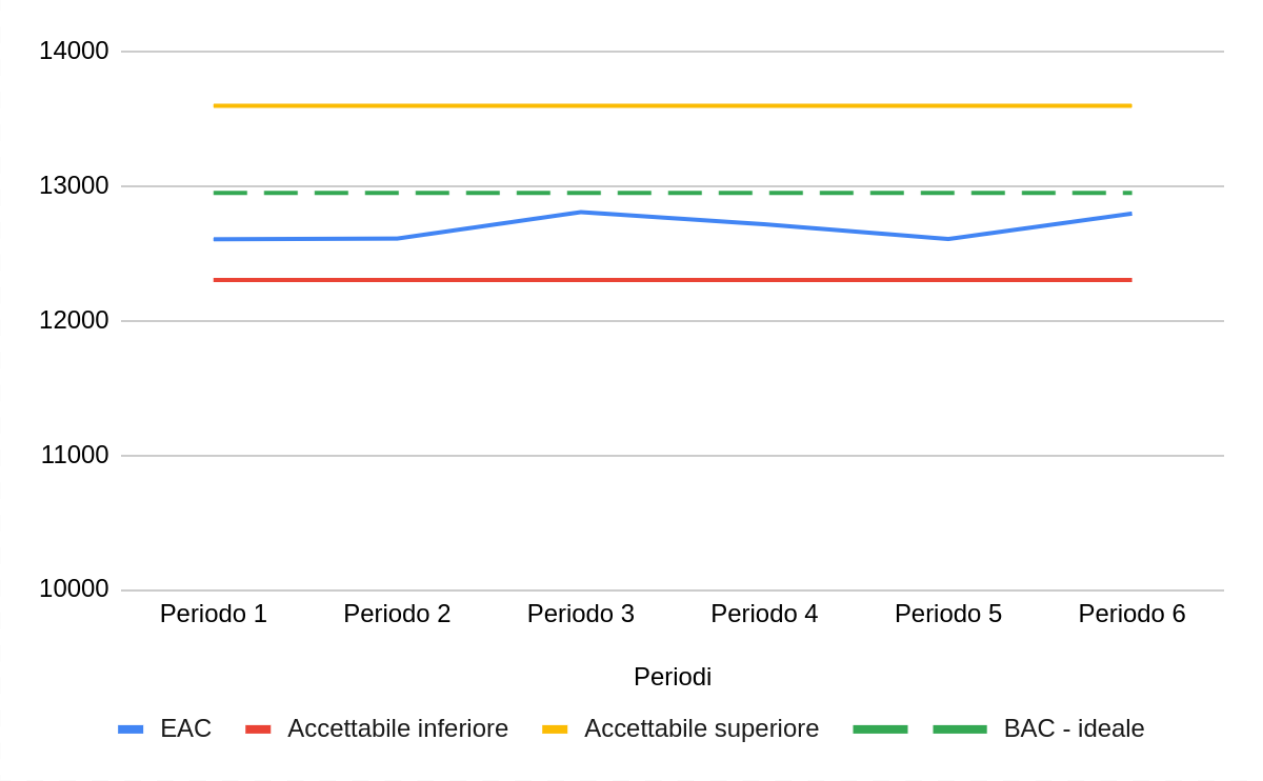
\includegraphics[width=0.9\linewidth]{EAC.png}
  \caption{Grafico a linee della metrica EAC}
  \label{fig:EACchart}
\end{figure}


\textbf{RTB}: Il grafico rappresenta la stima aggiornata del costo totale del progetto$_G$ al completamento. Questo valore è quindi determinato dalla somma 
dei costi sostenuti fino a un certo momento (in termini di ore produttive svolte), e dei costi stimati al completamento (in termini di ore produttive 
restanti in riferimento al preventivo iniziale del progetto$_G$).\\ 
In questo caso emerge dal grafico che il valore di EAC$_G$ è poco al di sotto del preventivo iniziale (BAC), e in ogni caso entro i valori accettabili definiti
per la metrica. Questo indica che il progetto$_G$ è sufficientemente in linea con le aspettative in termini di costi.\\

\noindent
\textbf{PB}: Per quanto riguarda la Product Baseline$_G$, il valore di EAC$_G$ si è sempre mantenuto entro i valori accettabili e poco al di sotto del valore ideale,
corrispondente al preventivo iniziale (BAC). Questo indica che il progetto$_G$ è in linea con le aspettative in termini di costi, e che anzi le spese previste sono sempre
state leggermente al di sotto della stima iniziale di 12.950,00 €.\\
Anche relativamente all'EAC dell'ultimo sprint$_G$ (undicesimo) che corrisponde all'effettiva spesa sostenuta dal gruppo, il valore registrato è di 12.510,00 €, e pertanto
il gruppo può affermare di aver risparmiato 440,00 € rispetto al budget iniziale.\\


\subsubsection{MPC05 - Planned Value (PV) \& MPC04 - Earned Value (EV)}

\begin{figure}[H]
  \centering
  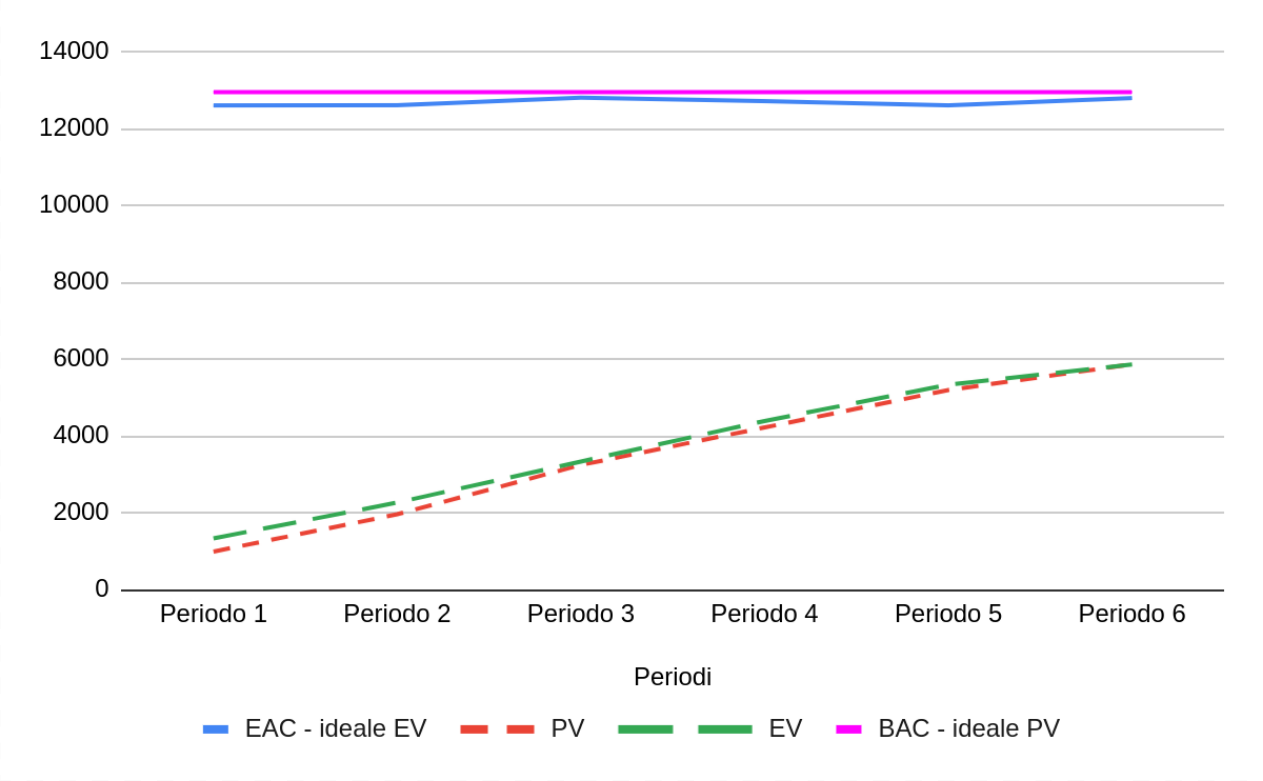
\includegraphics[width=0.9\linewidth]{EV-PV.png}
  \caption{Grafico a linee delle metriche EV e PV}
  \label{fig:EV-PVchart}
\end{figure}

\textbf{RTB}: Il grafico mostra la curva del valore guadagnato (Earned Value), e la curva del valore pianificato (Planned Value). Come si può notare osservando la 
figura le due curve sono molto vicine, questo indica che il lavoro effettivamente svolto è conforme alla pianificazione; e nello specifico quella dell'EV è sempre 
leggermente superiore a quella del PV$_G$. Ciò indica che il progetto$_G$ sta producendo un valore maggiore rispetto a quanto pianificato, e quindi che il lavoro svolto 
è leggermente al di sopra delle aspettative.\\

\noindent
\textbf{PB}: In questo caso le osservazioni già fatte per la RTB$_G$ si possono applicare anche alla PB$_G$: il lavoro effettivamente svolto (EV - Earned Value) è sempre stato 
conforme a quello pianificato (PV - Planned Value), e nello specifico il valore dell'EV è sempre stato leggermente superiore a quello del PV$_G$, confermando che il 
progetto$_G$ ha prodotto un valore maggiore rispetto a quanto pianificato.\\



\subsubsection{MPC03 - Actual Cost (AC) \& MPC02 - Estimate to Complete (ETC)}

\begin{figure}[H]
  \centering
  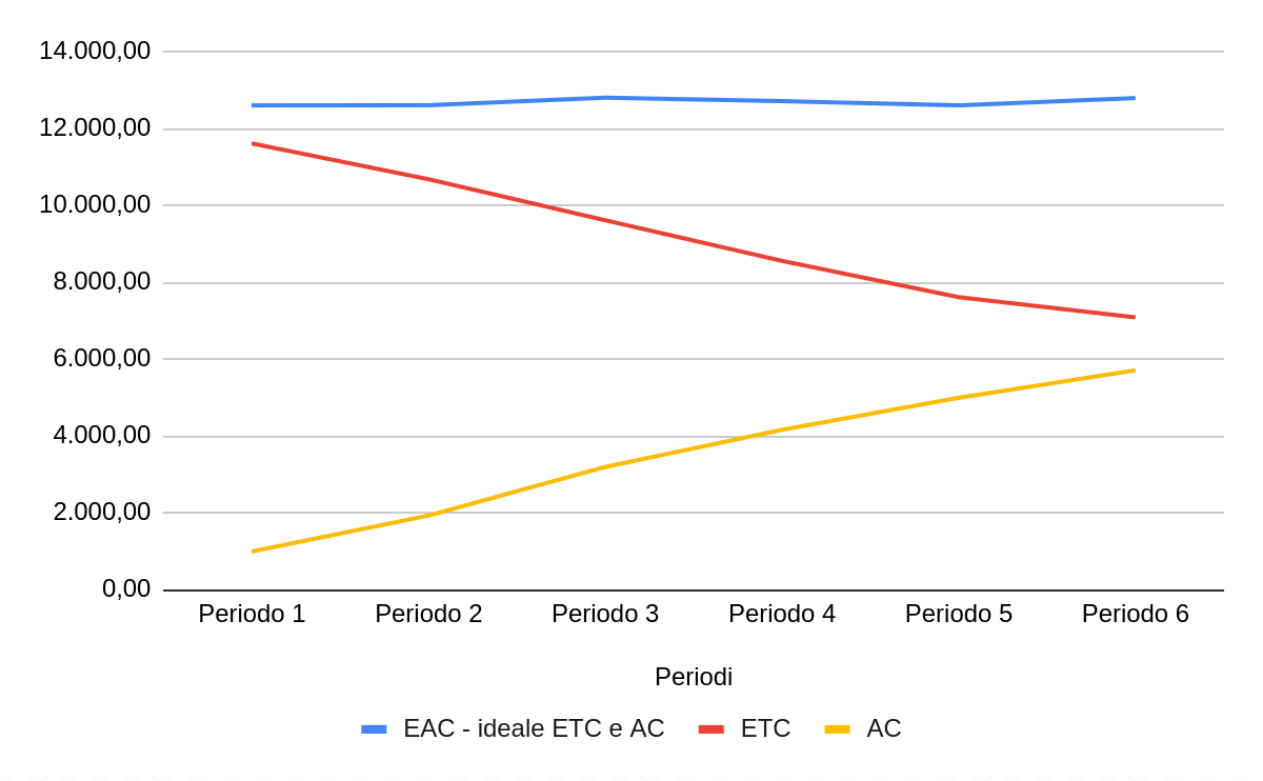
\includegraphics[width=0.9\linewidth]{AC-ETC.png}
  \caption{Grafico a linee delle metriche AC e ETC}
  \label{fig:AC-ETCchart}
\end{figure}

\textbf{RTB}: Il grafico rappresenta l'Actual Cost (AC), ovvero i costi sostenuti per portare il progetto$_G$ al suo stato corrente, e l'Estimate to Complete (ETC), 
cioè la stima del costo rimanente da sostenere per completare il progetto$_G$ per ogni periodo di misurazione (termine sprint$_G$). Entrambe le metriche hanno valore ideale
inferiore all'EAC, che viene rispettato in ogni iterazione.\\
Ovviamente l'ETC tende a diminuire al progredire del progetto$_G$ poiché questo si avvicina alla sua conclusione, mentre l'AC mostra una crescita proporzionale e inversa 
rispetto all'ETC, in linea con le aspettative economiche del progetto$_G$.\\

\noindent
\textbf{PB}: L'andamento lineare delle due metriche emerso in fase RTB$_G$ è riconfermato dal grafico anche in fase PB$_G$, e testimonia che al crescere delle spese sostenute 
(AC - Actual Cost), la stima delle spese da sostenere (ETC - Estimate to Complete) è sempre diminuita in maniera proporzionale e inversa.\\


\subsubsection{MPC08 - Cost Performance Index (CPI)}

\begin{figure}[H]
  \centering
  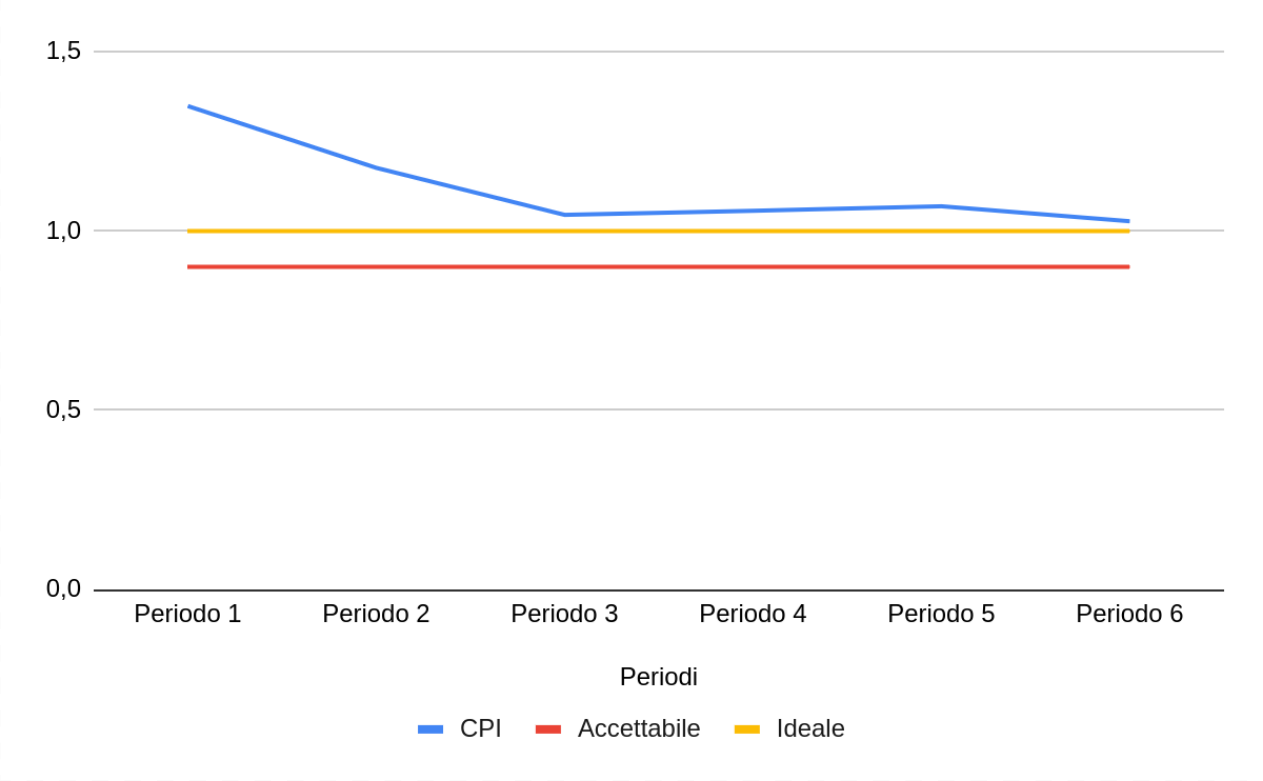
\includegraphics[width=0.9\linewidth]{CPI.png}
  \caption{Grafico a linee della metrica CPI}
  \label{fig:CPIchart}
\end{figure}

\textbf{RTB}: Il Cost Performance Index (CPI) è una metrica che indica quanti obiettivi sono stati raggiunti rispetto alle spese sostenute in un certo momento del
progetto$_G$. La metrica è data dal rapporto fra il valore guadagnato (EV) e i costi sostenuti (AC), e infatti il suo valore ideale deve essere maggiore o pari a 1.
Il valore accettabile invece è stato scelto essere maggiore o uguale a 0.9.\\
Il grafico mostra che il CPI$_G$ ha avuto valore strettamente maggiore di 1 per tutto il progetto$_G$, assestandosi fra il terzo e il sesto sprint$_G$ a un valore pari a circa 1.06.
Questo indica che il progetto$_G$ ha prodotto un valore maggiore rispetto ai costi sostenuti.\\

\noindent
\textbf{PB}: Anche nel corso della seconda fase del progetto$_G$ la metrica CPI$_G$ ha continuato il suo andamento, mantenendosi su un valore di poco superiore a 1.00, ovvero 
al di sopra della soglia del valore ideale. Questo indica che per l'intera durata della seconda fase del progetto$_G$ il gruppo ha prodotto un valore maggiore rispetto ai 
costi sostenuti.\\


% originariamente qui c'era una sottosezione in più di Pianificazione, che non appare però negli Obiettivi Metrici di qualità (sopra):
% \subsection{Qualità di processo$_G$ - Pianificazione}
% si può rimettere aggiungendo però pianificazione anche nei Obiettivi Metrici di qualità, e volendo inserendo in pianificazione anche la metrica proposta sotto a questa:
\subsubsection{MPC07 - Cost Variance (CV) \& MPC06 - Schedule Variance (SV)}

\begin{figure}[H]
  \centering
  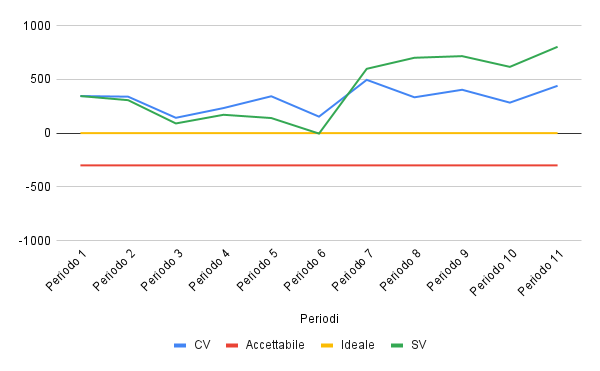
\includegraphics[width=0.9\linewidth]{CV-SV.png}
  \caption{Grafico a linee delle metriche CV e SV}
  \label{fig:CV-SVchart}
\end{figure}

\textbf{RTB}: Il grafico mostra l'andamento  della Cost Variance (CV) e della Schedule Variance (SV), che rappresentano rispettivamente: 
la differenza tra il valore guadagnato (EV) e i costi sostenuti (AC) e la differenza tra il valore guadagnato (EV) e il valore pianificato (PV).\\
La CV$_G$ resta sempre positiva per l'intera durata del progetto$_G$ fino al sesto sprint$_G$, e ciò indica che le spese effettuate sono inferiori rispetto al valore prodotto
dal team nel corso della prima parte del progetto$_G$.\\
La SV$_G$ mostra un andamento positivo fino al quinto sprint$_G$, e ciò indica che il gruppo ha saputo produrre un valore maggiore di quanto
pianificato nel corso delle iterazioni effettuate. Invece per il sesto sprint$_G$ la SV$_G$ è andata ad un valore non positivo.\\
% Possibile aggiunta di una metrica PV$_G$ - AC$_G$ per mostrare gli errori di pianificazione nei preventivi. Bisognerebbe però aggiungere questa metrica anche nelle NdP

\noindent
\textbf{PB}: Nel corso della seconda fase del progetto$_G$ la metrica CV$_G$ (Cost Variance) ha, anche in questo caso, mostrato un andamento nettamente positivo, dimostrando
che le spese sostenute sono sempre state inferiori rispetto al valore effettivamente prodotto dal team.\\
Per quanto riguarda invece la metrica SV$_G$ (Schedule Variance), il suo andamento è stato molto positivo (e in realtà anche significativamente superiore alla CV$_G$) per l'intera durata
della seconda fase del progetto$_G$. Questo indica che il gruppo ha saputo produrre un valore maggiore di quanto pianificato nel corso delle iterazioni effettuate.\\
Dall'osservazione delle due metriche messe a confronto emerge però che anche per la seconda fase del progetto$_G$, il gruppo ha spesso stimato preventivi di spesa superiori
rispetto ai consuntivi effettivamente registrati, fallendo nel rimediare a questa mancanza già osservata nella prima fase del progetto$_G$.\\



\subsection{Qualità di processo - Sviluppo}
\subsubsection{MPC10 - Requirements Stability Index (RSI)}

\begin{figure}[H]
  \centering
  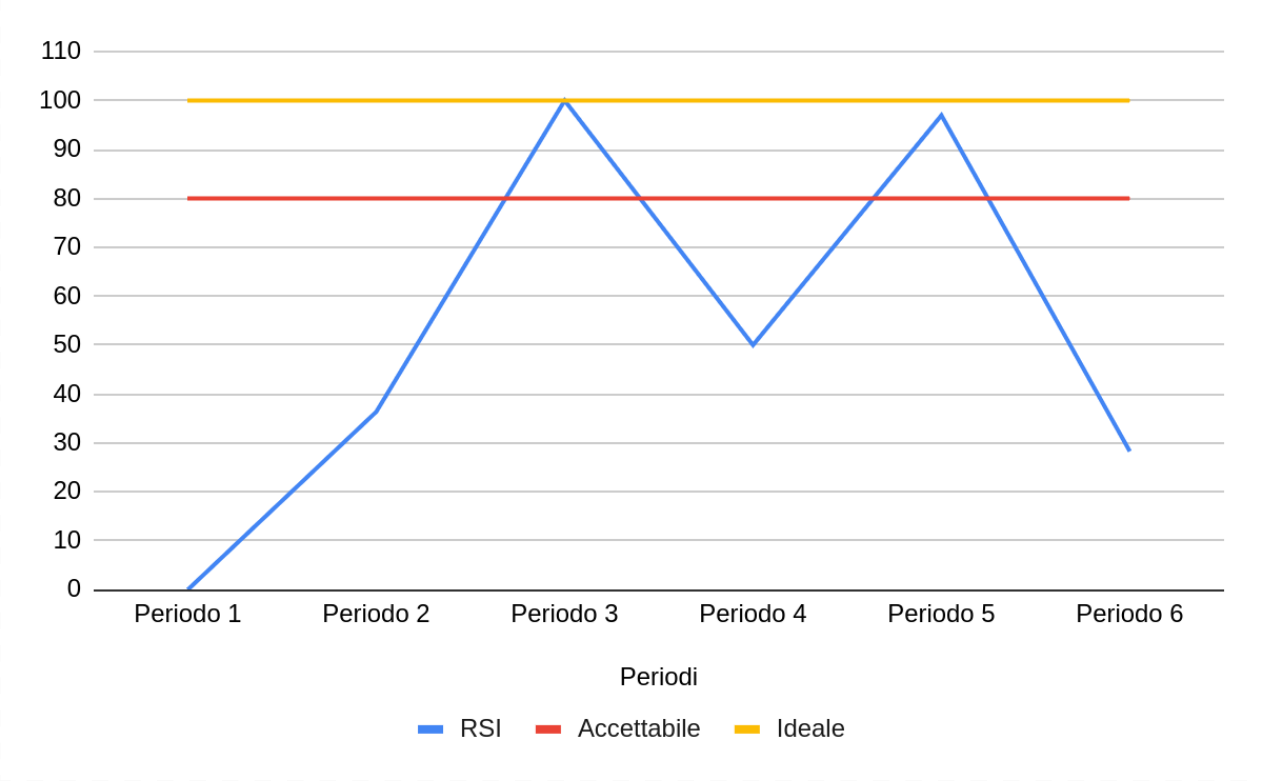
\includegraphics[width=0.9\linewidth]{RSI.png}
  \caption{Grafico a linee della metrica RSI}
  \label{fig:RSIchart}
\end{figure}

\textbf{RTB}: La metrica RSI$_G$ rappresenta un indice di stabilità dei requisiti individuati nel corso del progetto$_G$. Questo indice è in percentuale e assume valore tanto più alto 
quanto maggiore è la stabilità dei requisiti. In altre parole, il valore è alto se pochi requisiti sono cambiati rispetto all'ultima misurazione, mentre è basso se molti requisiti sono
stati modificati, aggiunti o rimossi rispetto all'ultima misurazione.\\
Come si può evincere dal grafico, l'RSI è partito da valore nullo (in maniera coerente rispetto alla formula usata per il calcolo di tale metrica, poiché nel primo sprint$_G$ 
sono stati definiti i primi requisiti); crescendo nella seconda iterazione (mentre il primo tentativo di identificazione dei requisiti era ancora in corso); e ha poi mostrato 
un andamento altalenante, con picchi di stabilità nel terzo e quinto periodo e cali significativi (inferiori al valore accettabile) in corrispondenza della terza e sesta iterazione. In entrambi questi 
casi il valore basso è seguito a significative modifiche dei requisiti, successive a degli incontri di chiarimento organizzati con il professor Cardin, che  hanno 
evidenziato degli errori nell'approccio del gruppo all'analisi dei requisiti.\\
Complessivamente il gruppo si aspetta una maggiore stabilità in futuro, in caso di un buon esito della revisione RTB$_G$, mentre potrebbero essere necessari ulteriori
significativi cambiamenti in caso di esito negativo.\\

\noindent
\textbf{PB}: Dall'analisi del grafico della metrica RSI$_G$ (Requirements Stability Index) emerge che il valore di stabilità dei requisiti è sempre stato entro la soglia accettabile
per tutta la durata della seconda fase del progetto$_G$, con delle leggere discese (sempre superiori alla soglia di accettazione) in corrispondenza del settimo e nono periodo, in cui si sono
concentrati i maggiori sforzi da parte del gruppo di correggere le imprecisioni individuate nell'\textit{Analisi\_dei\_Requsisitiv1.0.0} dal professor Cardin.\\


\subsection{Qualità di processo - Gestione dei processi}
\subsubsection{MPC16 - Rischi non previsti}

\begin{figure}[H]
  \centering
  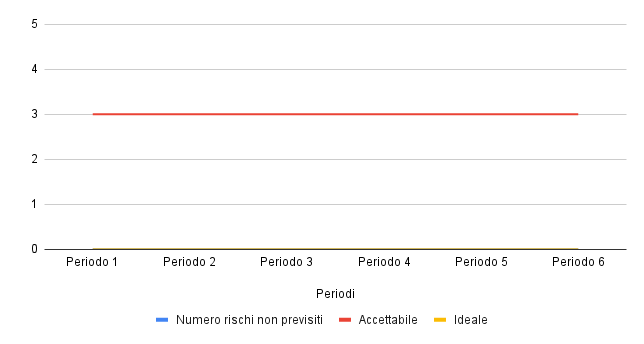
\includegraphics[width=0.9\linewidth]{RNP.png}
  \caption{Grafico a linee della metrica "Rischi non previsti"}
  \label{fig:RNPchart}
\end{figure}

\textbf{RTB}: Nel corso del progetto$_G$ il team ha senz'altro avuto modo di affrontare svariati dei rischi emersi durante l'analisi dei rischi, tuttavia non sono stati
riscontrati rischi non previsti nel corso dei primi sei periodi del progetto$_G$.\\

\noindent
\textbf{PB}: Anche durante la seconda fase del progetto$_G$ il gruppo non ha riscontrato alcun rischio$_G$ non previsto.\\


\subsubsection{MPC17 - Efficienza temporale (ET)}

\begin{figure}[H]
  \centering
  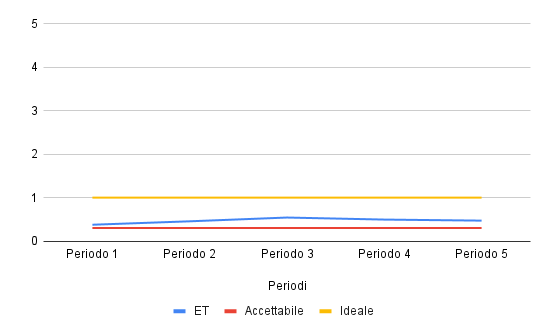
\includegraphics[width=0.9\linewidth]{ET.png}
  \caption{Grafico a linee della metrica ET}
  \label{fig:ETchart}
\end{figure}

% da modificare NdP aggiungendo il fatto che le ore produttive e totali si riferiscono al singolo sprint$_G$ e non all'interezza del progetto$_G$
\textbf{RTB}: La metrica di efficienza$_G$ temporale è data dal rapporto fra il numero di ore totali e produttive per ogni sprint$_G$, e indica quante delle ore dedicate al progetto$_G$
sono state effettivamente usate per la produzione di materiale (software o di altra natura), rispetto alle ore effettivamente consumate dai membri del gruppo. Le ore 
produttive sono state accuratamente rendicontate per l'intera durata del progetto$_G$, mentre quelle totali (che includono anche le produttive), sono state misurate in
maniera più precisa possibile, ma senza pretese di assoluta esattezza, per via della natura di queste ultime.\\
Dal grafico emerge che la ET si mantiene, per l'intera durata delle prime sei iterazioni del progetto$_G$,  al di sotto del valore massimo accettabile (pari a 5.0), ma al di 
sopra del valore ideale (pari a 1.0).\\

\noindent
\textbf{PB}: Da notare che rispetto alla prima fase del progetto$_G$, la formula di calcolo della metrica ET è stata modificata invertendo numeratore e denominatore, per 
renderla più facilmente interpretabile.\\
Detto ciò, per la seconda fase del progetto$_G$ il valore della metrica si è sempre attestato fra 2.5 e 3.0, in linea con le aspettative, ma senza registrare un miglioramento 
rispetto alle ultime iterazioni della prima fase.\\


\subsection{Qualità di processo - Documentazione}
\subsubsection{MPC01 - Errori ortografici}

\begin{figure}[H]
  \centering
  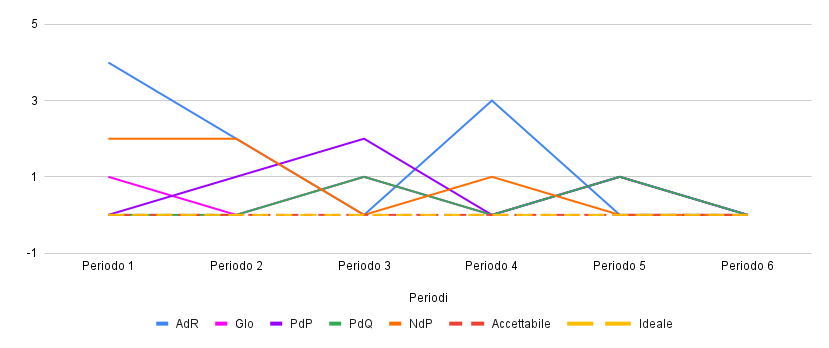
\includegraphics[width=0.9\linewidth]{EO.png}
  \caption{Grafico a linee della metrica "Errori ortografici"}
  \label{fig:EOchart}
\end{figure}

\textbf{RTB}: La metrica rappresenta un indice della qualità della documentazione$_G$ e fa riferimento al numero di errori ortografici individuati in fase di verifica 
dei documenti prodotti.\\
Sebbene il valore ideale non sia mai rispettato nel corso dei primi 5 sprint$_G$ per tutta la documentazione$_G$, è bene evidenziare che il team ha mantenuto comunque dei valori bassi, che hanno 
presentato dei prevedibili aumenti in fasi di grande produzione di documentazione$_G$. L'obiettivo del gruppo è comunque stato quello di consegnare al termine del sesto periodo
dei documenti privi di errori ortografici, e ciò è stato raggiunto, dato che almeno da parte nostra non ne sono stati individuati.\\

\noindent
\textbf{PB}: Da notare che, rispetto alla prima fase del progetto$_G$, lo stile del grafico è stato modificato da grafico a linee a grafico a barre, per rendere più chiara 
la lettura dei dati.\\
Anche nel corso di questa seconda fase del progetto$_G$ il gruppo ha mantenuto un numero di errori ortografici non conforme al valore accettabile per quasi 
tutte le iterazioni, riuscendo però a consegnare al termine del progetto$_G$ dei documenti quanto più possibile privi di errori ortografici. Anche in questo caso sono stati 
registrati valori più elevati in corrispondenza di periodi di grande produzione di documentazione$_G$ (sopratutto nel 10 sprint$_G$).


\subsubsection{MPC11 - Indice Gulpease}

\begin{figure}[H]
  \centering
  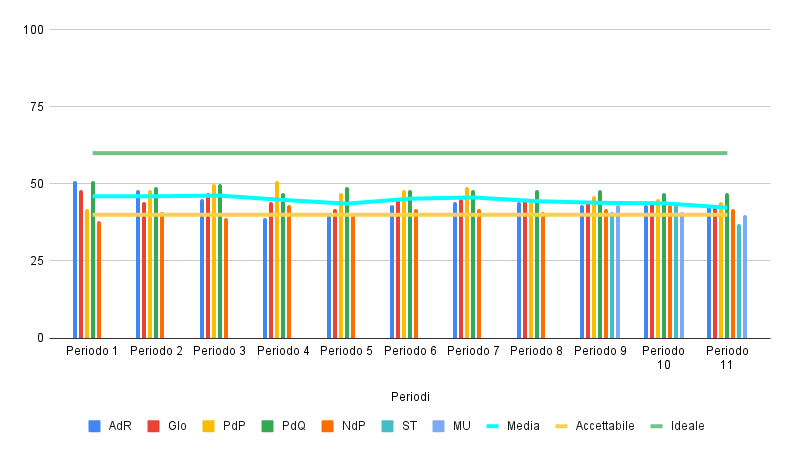
\includegraphics[width=0.9\linewidth]{gulpease.png}
  \caption{Grafico a linee della metrica "Indice di Gulpease"}
  \label{fig:gulpease_chart}
\end{figure}

\textbf{RTB}: Emerge da un'analisi del grafico che il valore di accettazione dell'indice di Gulpease (valore ideale $geq$ 60; valore accettabile $geq$ 40), è stato quasi sempre rispettato in tutti i documenti
redatti per cui si è scelto di misurarlo; con alcune eccezioni per il documento \textit{Analisi dei Requisiti} (nel quarto periodo), e per il documento \textit{Norme di Progetto} (nella prima e nella terza iterazione).\\
Appare tuttavia chiaro che il gruppo ha avuto non poche difficoltà a raggiungere il valore ideale per questa metrica, poiché è stata sottovalutata la difficoltà dello 
scrivere documentazione$_G$ chiara e con linguaggio semplice.\\
A questo proposito il gruppo si porrà in futuro l'obiettivo di migliorare il valore di questa metrica, cercando di esprimere i concetti con frasi più brevi e semplici.\\

\noindent
\textbf{PB}: Da notare che lo stile del grafico è stato modificato da grafico a linee a grafico a barre e linee, per rendere più chiara l'interpretazione dei dati.\\
Relativamente alla seconda fase del progetto$_G$ il gruppo ha registrato un andamento della metrica analogo a quello della prima fase, con un valore leggermente 
più basso rispetto alla prima fase.\\
Malgrado ciò il valore accettabile risulta rispettato sia per la media, che per quasi tutti i singoli documenti, ad eccezione del documento \textit{Specifica\_Tecnicav1.0.0}, 
per la quale, nell'undicesimo periodo si è registrato un valore pari a 37 (leggermente al di sotto della soglia accettabile).\\


\subsection{Qualità di processo - Gestione della qualità}
\subsubsection{MPC15 - Metriche di qualità soddisfatte}

\begin{figure}[H]
  \centering
  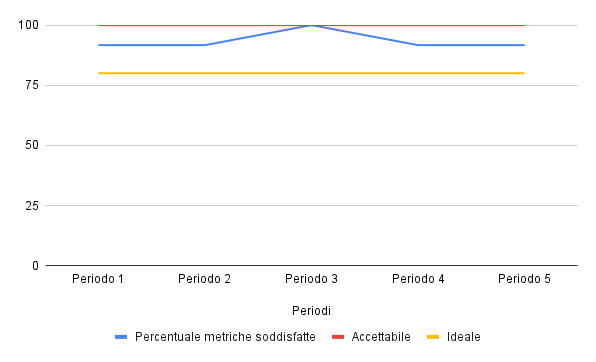
\includegraphics[width=0.9\linewidth]{metricheRispettate.png}
  \caption{Grafico a linee della metrica "metriche di qualità soddisfatte"}
  \label{fig:metricheRispettate_chart}
\end{figure}

\textbf{RTB}: Questa metrica rispecchia la capacità del team di rispettare i valori accettabili delle altre metriche misurata nel corso del progetto$_G$. Dall'analisi del suo 
grafico emerge che il gruppo è sempre riuscito a garantire il rispetto di più dell'90\% delle metriche misurate. Ciò è un segnale chiaramente positivo che dimostra
un buon lavoro del gruppo dal punto di vista della gestione della qualità.\\
Detto ciò è però bene notare che il gruppo, in solo uno dei precedenti sei periodi, ha raggiunto il valore ideale (100\%), quindi ci sono comunque importanti margini
di miglioramento da perseguire.\\
Un'ultima nota va aggiunta per specificare che il gruppo ha scelto di considerare la metrica relativa all'indice di Gulpease, che si applica a cinque documenti distinti, come 
una metrica unica facendo la media dei cinque valori misurati.\\

\noindent
\textbf{PB}: Anche nel corso della seconda fase del progetto$_G$ il gruppo ha sempre rispettato il valore accettabile della metrica, anche se il minimo storico (pari a 87,5\%)
è stato registrato in corrispondenza della ottava iterazione.\\
Anche in questo caso il gruppo non è riuscito a mantenere un valore costante pari al 100\%, ma ha comunque raggiunto tale valore ideale in corrispondenza degli ultimi
due sprint$_G$ del progetto$_G$.\\



\subsection{Qualità di processo - Analisi dei requisiti}
\subsubsection{MPC09 - Requisiti Obbligatori Soddisfatti (ROS)}

\begin{figure}[H]
  \centering
  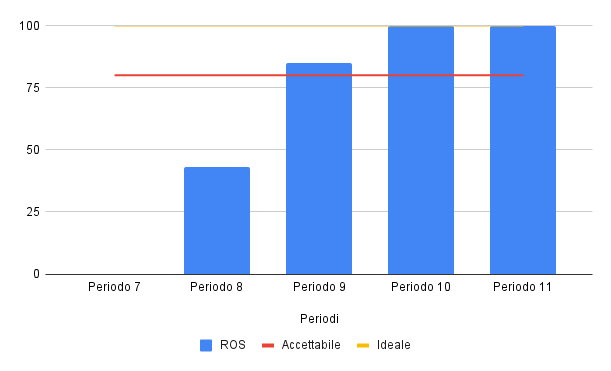
\includegraphics[width=0.9\linewidth]{ROS.png}
  \caption{Grafico a linee della metrica ROS}
\end{figure}

\textbf{PB}: Questa metrica riflette la percentuale di requisiti obbligatori soddisfatti durante ogni iterazione. Analizzando il grafico emerge che nel periodo 7 (in cui il
gruppo aveva iniziato la progettazione ma non la codifica) il valore della metrica non è stato considerato. Dal periodo successivo sono iniziate le misurazioni, che 
hanno mostrato un valore inizialmente basso (circa 40\%) in corrispondenza della ottava iterazione (poiché il codice era ancora incompleto), e un andamento crescente, 
con valori positivi nelle successive tre iterazioni.\\
La costante progressione verso il 100\% dei requisiti obbligatori soddisfatti, culminata nel raggiungimento del valore ideale, è un segnale estremamente positivo. 
Dimostra una solida comprensione delle esigenze del progetto$_G$ e un'efficace esecuzione da parte del team nel tradurre tali requisiti in funzionalità complete.


\subsection{Qualità di processo - Verifica}
\subsubsection{MPD04 - Line Coverage}

\begin{figure}[H]
  \centering
  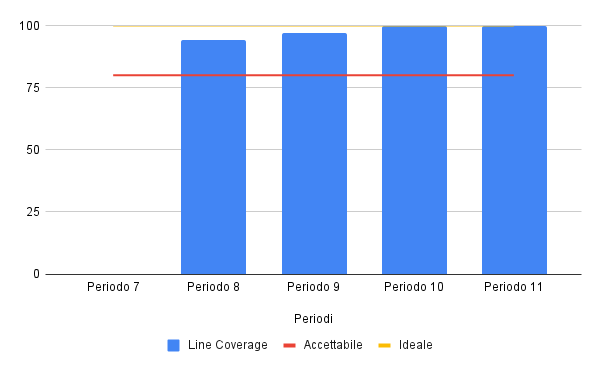
\includegraphics[width=0.9\linewidth]{LineCoverage.png}
  \caption{Grafico a linee della metrica "Line coverage"}
\end{figure}

\textbf{PB}: La metrica rappresenta la percentuale di linee di codice coperte dai test$_G$ automatici. Il valore ideale è 100\%, mentre il valore accettabile è 90\%.\\
Il grafico mostra che il valore di questa metrica è sempre stato al di sopra del valore accettabile, e ha raggiunto il valore ideale in prossimità della revisione PB$_G$.\\
Da notare che non è presente alcun valore registrato in corrispondenza della settima iterazione poiché nessun test$_G$ era ancora stato implementato durante quest'ultima.\\


\subsubsection{MPD05 - Branch Coverage}

\begin{figure}[H]
  \centering
  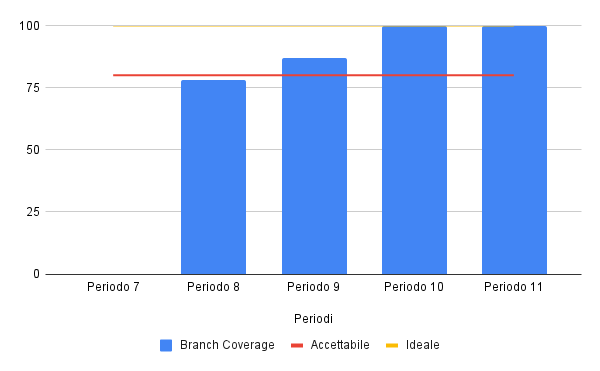
\includegraphics[width=0.9\linewidth]{BranchCoverage.png}
  \caption{Grafico a linee della metrica "Branch coverage"}
\end{figure}

\textbf{PB}: La metrica rappresenta la percentuale di rami di codice coperti dai test$_G$ automatici. Il valore ideale è 100\%, mentre il valore accettabile è 90\%.\\
Il grafico mostra che il valore di questa metrica è sempre stato al di sopra del valore accettabile, e ha raggiunto il valore ideale in prossimità della revisione PB$_G$.\\
Da notare che non è presente alcun valore registrato in corrispondenza della settima iterazione poiché nessun test$_G$ era ancora stato implementato durante quest'ultima.\\


\subsubsection{MPD09 - Linee di codice per metodo}

\begin{figure}[H]
  \centering
  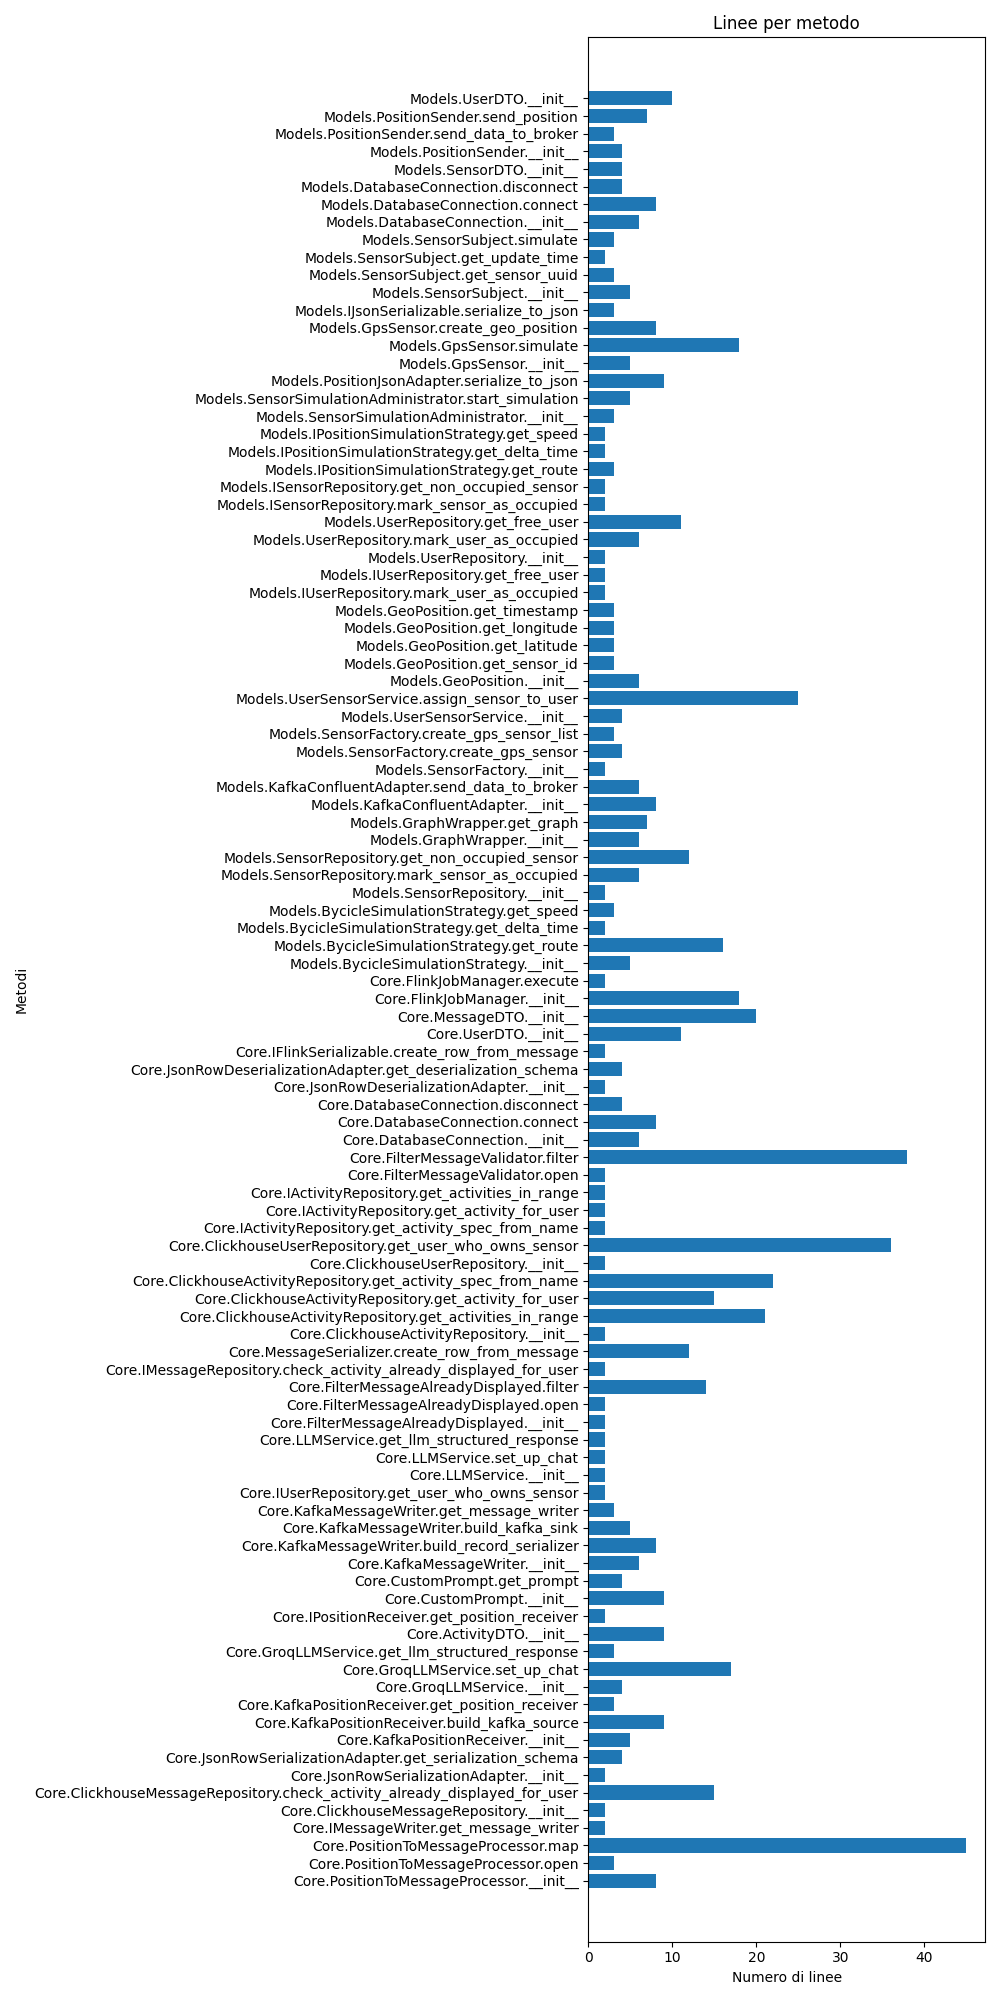
\includegraphics[width=0.7\linewidth]{metrics_lines.png}
  \caption{Grafico a barre della metrica "Linee di codice per metodo"}
\end{figure}

\textbf{PB}: Questo grafico rappresenta il numero di linee di codice per ciascun metodo scritto durante la fase di codifica.\\
Rispetto alla maggior parte delle altre metriche il grafico non rappresenta un andamento temporale, ma mostra il numero di linee di codice per ogni metodo allo stato
corrente del prodotto software; ciò perché non sarebbe stato possibile rappresentare in maniera immediata e  facilmente leggibile tale metrica altrimenti.\\
In ogni caso dal grafico si evince che il valore ideale (inferiore a 25) è quasi sempre stato rispettato, ad esclusione di tre casi, in cui è comunque stato registrato
un valore accettabile (inferiore a 50).\\


% \subsubsection{MPD11 - Parametri per metodo}

% \begin{figure}[H]
%   \centering
%   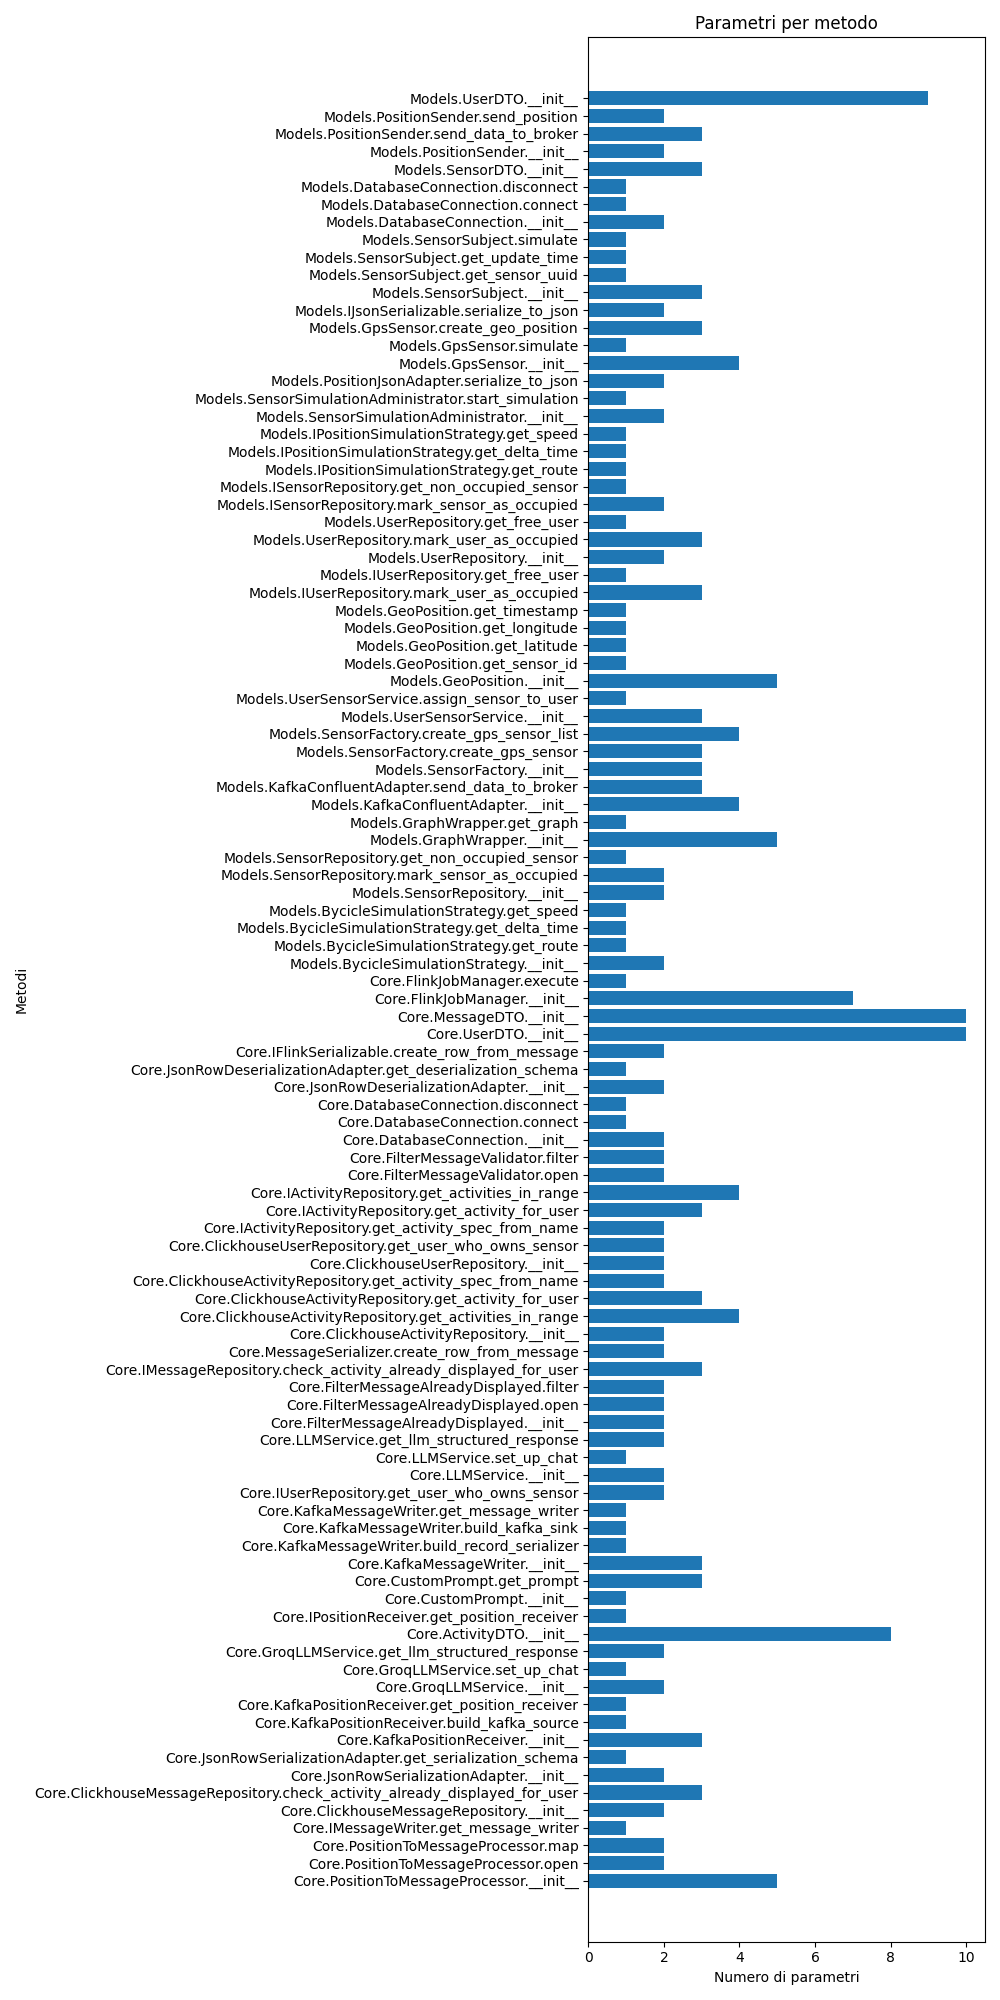
\includegraphics[width=0.9\linewidth]{metrics_parameters.png}
%   \caption{Grafico a barre della metrica "Parametri per metodo"}
% \end{figure}

% \textbf{PB}:


\subsubsection{MPD10 - Attributi per classe}

\begin{figure}[H]
  \centering
  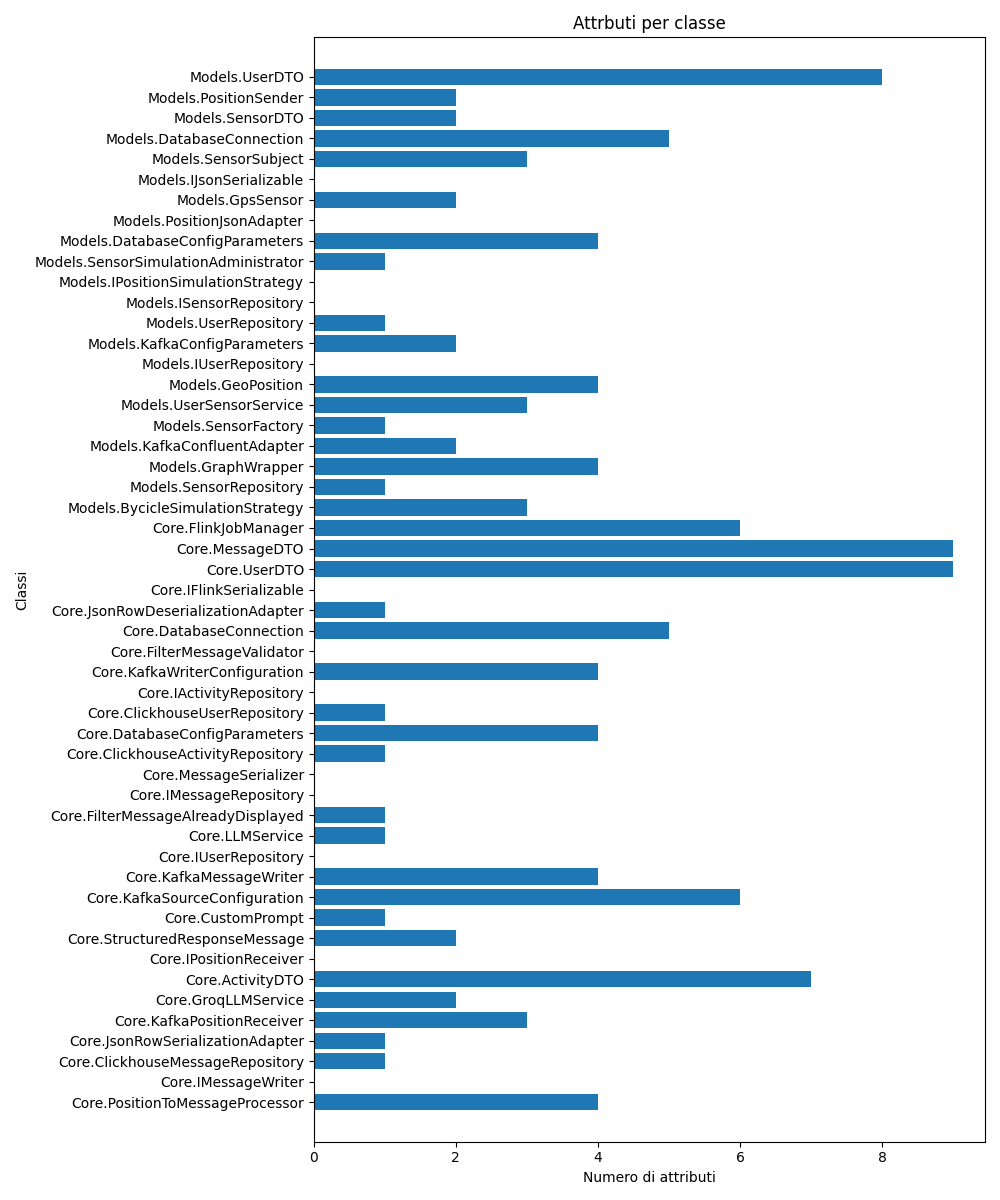
\includegraphics[width=0.9\linewidth]{metrics_attributes.png}
  \caption{Grafico a barre della metrica "Attributi per classe"}
\end{figure}

\textbf{PB}: Questo grafico rappresenta il numero di attributi per ogni classe scritta durante la fase di codifica.\\
Rispetto alla maggior parte delle altre metriche il grafico non rappresenta un andamento temporale, ma mostra il numero di attributi per ogni classe allo stato 
corrente del prodotto software; ciò perché non sarebbe stato possibile rappresentare in maniera immediata e  facilmente leggibile tale metrica altrimenti.\\
Analizzando il grafico si evince che il valore ideale (inferiore a 5) è sempre stato rispettato, ad esclusione di un caso, in cui è comunque stato registrato un valore
accettabile (inferiore a 7).\\


\subsubsection{MPD11 - Structure Fan IN}

\begin{figure}[H]
  \centering
  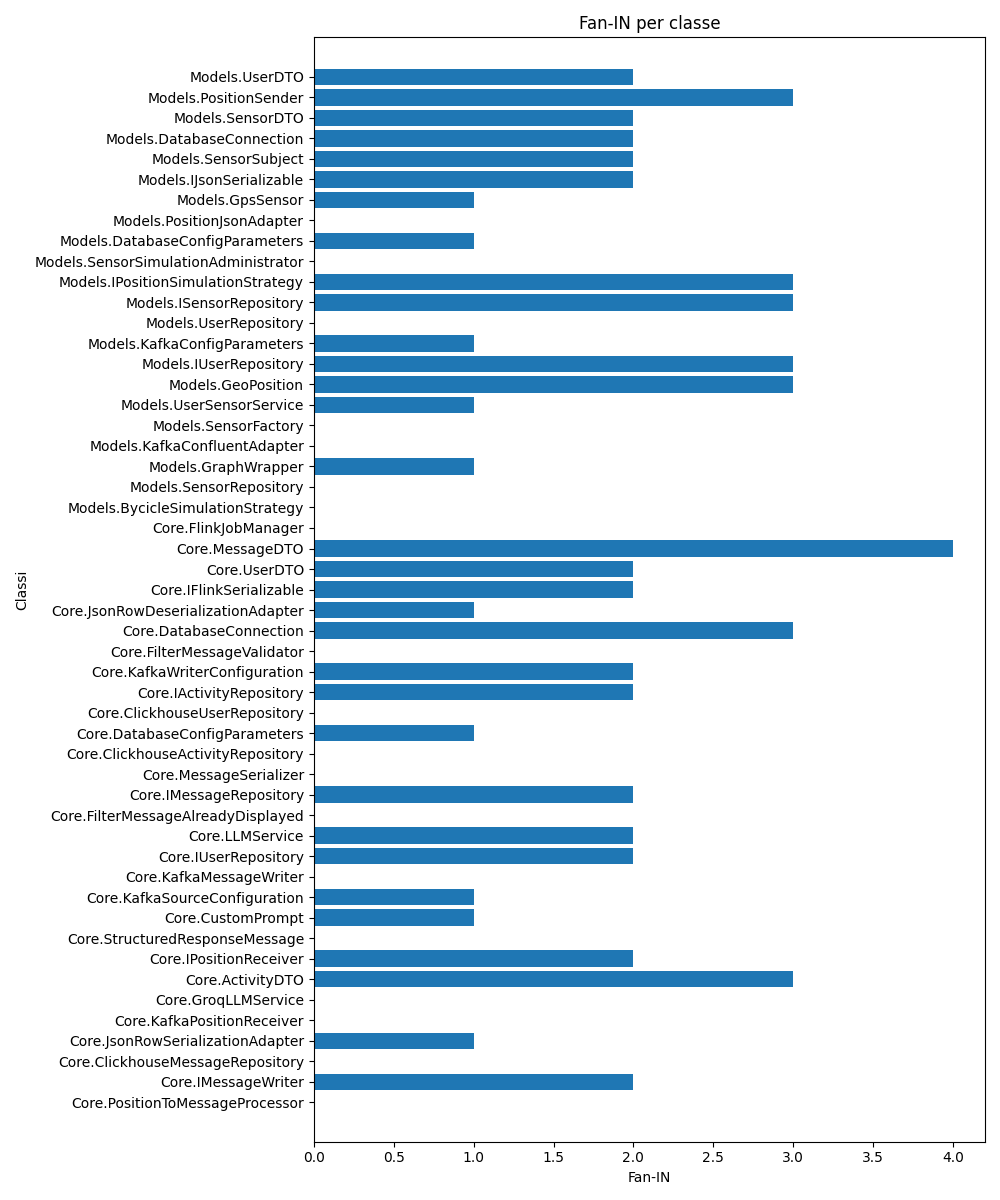
\includegraphics[width=0.9\linewidth]{metrics_fan_in.png}
  \caption{Grafico a barre della metrica "Structure Fan IN"}
\end{figure}

\textbf{PB}: Questo grafico rappresenta per ogni classe il numero di altre classi che dipendono da essa.\\
Rispetto alla maggior parte delle altre metriche il grafico non rappresenta un andamento temporale, ma mostra il valore di fan-IN per ogni classe allo stato 
corrente del prodotto software; ciò perché non sarebbe stato possibile rappresentare in maniera immediata e  facilmente leggibile tale metrica altrimenti.\\
Dall'analisi del grafico emerge che la fan-IN è sempre stata inferiore a 5 e per molti moduli si è registrato un valore nullo. Questa metrica non ha un valore ideale,
poiché un alta fan-IN indica che una classe è molto utilizzata da altre classi, e quindi è un buon segnale di riutilizzo del codice; ma allo stesso tempo un valore 
elevato indica che una classe crea molto accoppiamento essendo molto utilizzata, e quindi è un segnale negativo.\\ In generale i valori riscontrati non sono troppo 
elevati, e sono in linea con le aspettative del gruppo.\\


\subsubsection{MPD12 - Structure Fan OUT}

\begin{figure}[H]
  \centering
  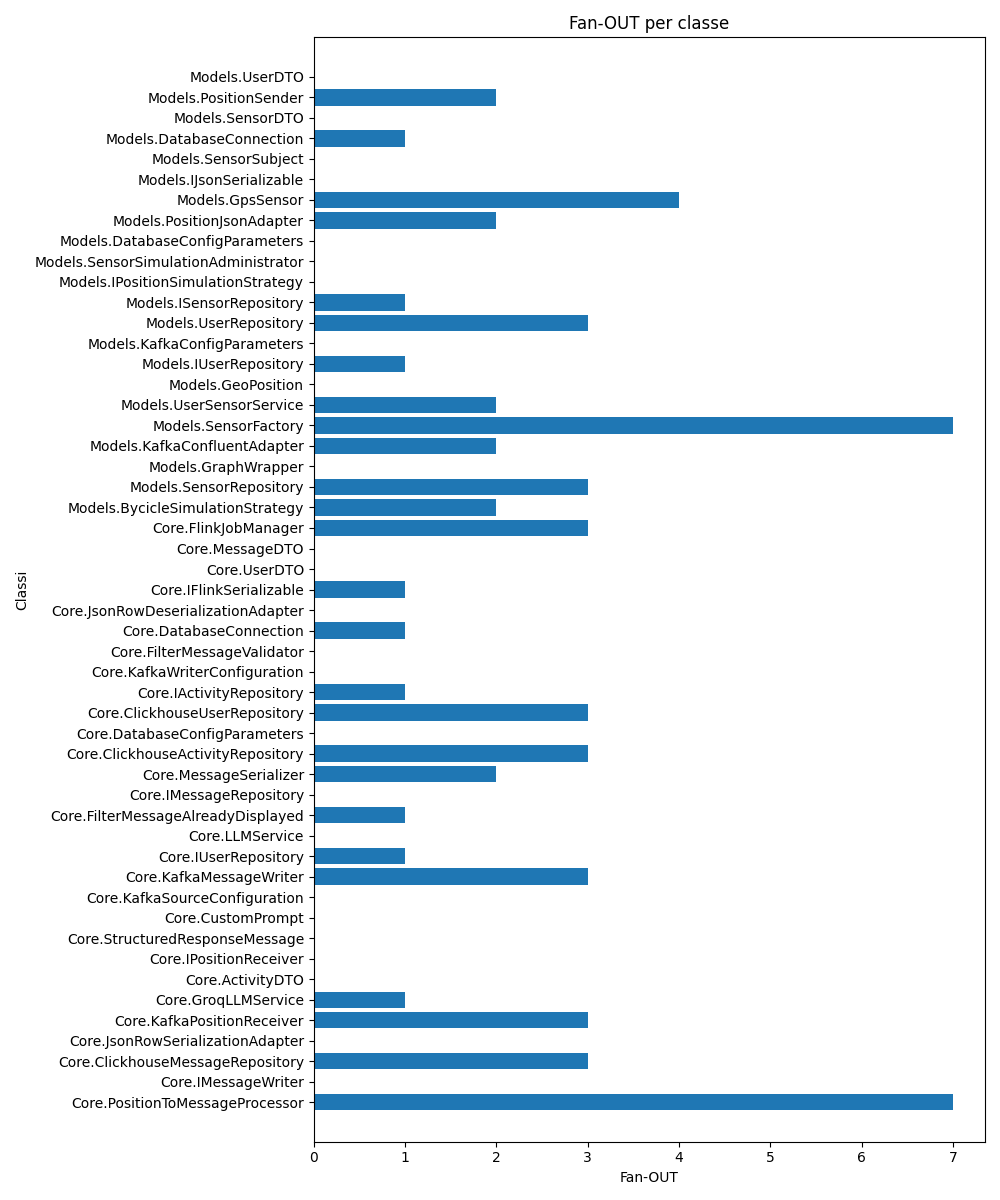
\includegraphics[width=0.9\linewidth]{metrics_fan_out.png}
  \caption{Grafico a barre della metrica "Structure Fan OUT"}
\end{figure}

\textbf{PB}: Questo grafico rappresenta per ogni classe il numero di altre classi la prima chiama o usa.\\
Rispetto alla maggior parte delle altre metriche il grafico non rappresenta un andamento temporale, ma mostra il valore di fan-OUT per ogni classe allo stato 
corrente del prodotto software; ciò perché non sarebbe stato possibile rappresentare in maniera immediata e  facilmente leggibile tale metrica altrimenti.\\
Dall'analisi del grafico emerge che la fan-OUT è sempre stata inferiore a 7 e per molti moduli si è registrato un valore nullo. Questa metrica non ha un valore ideale,
poiché un alta fan-OUT indica che una classe è molto dipendente da altre, cosa che generalmente è negativa (a meno che la classe non sia un controller o orchestratore); 
ma allo stesso tempo un valore basso, anche se p indice di buona coesione e indipendenza, può anche indicare che una classe è troppo semplice o superflua.\\
In generale il valore di fan-OUT ad eccezione di alcuni casi, è stato relativamente basso, in linea con le aspettative del gruppo.\\


\subsubsection{MPC14 - Passed test cases percentage}

\begin{figure}[H]
  \centering
  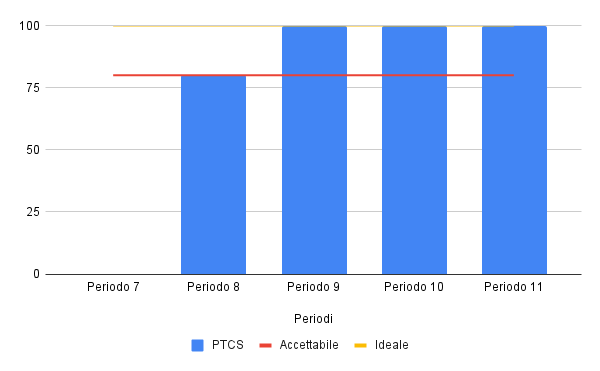
\includegraphics[width=0.9\linewidth]{PTCP.png}
  \caption{Grafico a linee della metrica "Passed test cases percentage"}
\end{figure}

\textbf{PB}: Questa metrica rappresenta la percentuale di test$_G$ superati rispetto al totale dei test$_G$ eseguiti. Il valore ideale è 100\%, mentre il valore accettabile è 90\%.\\
Il grafico mostra che il valore di questa metrica è sempre stato al di sopra del valore accettabile, e ha raggiunto il valore ideale in prossimità della revisione PB$_G$.\\
Da notare che non è presente alcun valore registrato in corrispondenza della settima iterazione poiché nessun test$_G$ era ancora stato implementato durante quest'ultima.\\

\section{Metriche non incluse nel cruscotto}
Le seguenti metriche, pur essendo parte integrante della valutazione della qualità del prodotto, non sono state incluse nel cruscotto$_G$ di valutazione delle qualità. La loro natura non si presta infatti a una rappresentazione grafica.
Di seguito sono riportati i dettagli relativi a ciascuna metrica, con le rispettive soglie di accettazione e i valori attualmente rilevati.

\begin{table}[H]
  \centering
\begin{tabular}{|c|c|c|c|}
    \hline
    \textbf{Metrica} & \textbf{Descrizione} & \textbf{Valore accettazione} & \textbf{Valore attuale}\\
    \hline
    MPD06 & Tempo medio di risposta & $\leq$ 10 secondi & 2 secondi\\
    \hline
    MPD07 & Facilità di utilizzo & $\leq$ 7 click & 5 click\\
    \hline
    MPD08 & Tempo medio di apprendimento & $\leq$ 5 minuti & 3 minuti\\
    \hline
    MPD13 & Versioni browser supportati & $\geq$ 80\% & 100\% \\
    \hline
    \end{tabular}
    \caption{Metriche di qualità non incluse nel cruscotto}
\end{table}

\end{justify}
\end{document}
